%\documentclass[11pt,a4paper]{article}
\documentclass[11pt
  , a4paper
  , article
  , oneside
%  , twoside
%  , draft
]{memoir}

\usepackage{control}
\usepackage[numbers]{natbib}


\begin{document}

\newcommand{\technumber}{
  RAON Control-Document Series\\
  Revision : v0.1,   Release : Mar. 12. 2015}
\title{\textbf{EPICS와 SNMP 통합}}

\author{박미정\thanks{mijoy0909@ibs.re.kr} \\

  Rare Isotope Science Project\\
  Institute for Basic Science, Daejeon, South Korea
}
\date{\today}


\renewcommand{\maketitlehooka}{\begin{flushright}\textsf{\technumber}\end{flushright}}
%\renewcommand{\maketitlehookb}{\centering\textsf{\subtitle}}
%\renewcommand{\maketitlehookc}{C}
%\renewcommand{\maketitlehookd}{D}

\maketitle

\begin{abstract}
본 문서는 중이온가속기 제어의 기본 Framework이 되는 EPICS와 IP 네트워크상의 장비 관리 및 모니터링 프로토콜인 SNMP통합 및 모니터링 시스템의 구현에 대해 논한다.
\end{abstract}

\chapter{중이온가속기 제어 시스템}
가속기 제어 시스템은 사용자가 원하는 빔을 사용자가 원하는 장소로 효율적으로 보낼 수 있도록 가속기를 구성하는 모든 요소를 감시하며 원격으로 제어하는 장치 조직망이다. EPICS는 실시간 분산 제어 시스템이자 중이온가속기 제어의 기본 Framework로 중이온가속기 제어 시스템 개발에 사용된다. 

\section{중이온가속기}
한국의 기초과학연구원(Institute for Basic Science) 산하 중이온가속기구축사업단(Rare Isotope Science Project)은 빔에너지 200Mev/u, 빔 출력 400kW급 희귀동위 원소 가속기 시설을 구축하고 있다. 중이온가속기구축사업단은 수소, 헬륨보다 무거운 지구 상의 모든 원소의 이온을 빛의 속도에 가깝게 가속하는 가속기를 구축하는 연구시설로, 중이온가속기는 전기장을 이용해 중이온(탄소, 우라늄 등)을 빠른 속도로 가속하며, 이렇게 가속된 입자들을 표적 물질에 충동시켜 자연 상태에 존재하지 않는 다양한 희귀동위원소 생성에 이용하거나, 원자핵 등의 관찰, 물질의 성질 연구에 이용한다\citep{raon}\citep{risp}. 

\section{SNMP}
SNMP (Simple Network Management Protocol)\footnote{* SNMP에 관한 자세한 설명은 SNMP 이해 및 응답시간 테스트 문서를 참조 바란다}는 IP 네트워크 상의 장치 및 장비들을 관리하고 모니터링하기 위한 인터넷 표준 프로토콜이다\citep{snmp}. SNMP는 인증과 암호화 등의 차이로 v1/2c/3의 세 가지 버전으로 나뉘며, 그림\ref{fig:relationship_m_a}과 같이 Manager/Agent 구조이다\citep{snmpm_a}. Manager는 Agent에게 원하는 장비의 정보를 요청하며, 장비의 설정을 변경한다. Agent는 Manager가 요청한 장비의 정보를 제공하고, 시스템 충돌이나 재부팅 등의 장비에 영향을 미치거나 발생한 Event를 비동기적으로 알리기 위해 Trap 메시지를 보낸다. OID (Object Identifiers시 객체로 구성된 MIB (Management Information Base)는 계층구조를 이루며, 장비의 정보를 내포하고 있다. 일반적인 TCP/IP 관리정보는 MIB-2(RFC 1213)에 포함돼있고, 특정 장비들의 정보는 장비제조업체에서 제공한다. 

\begin{figure}[h!]
  \centering
  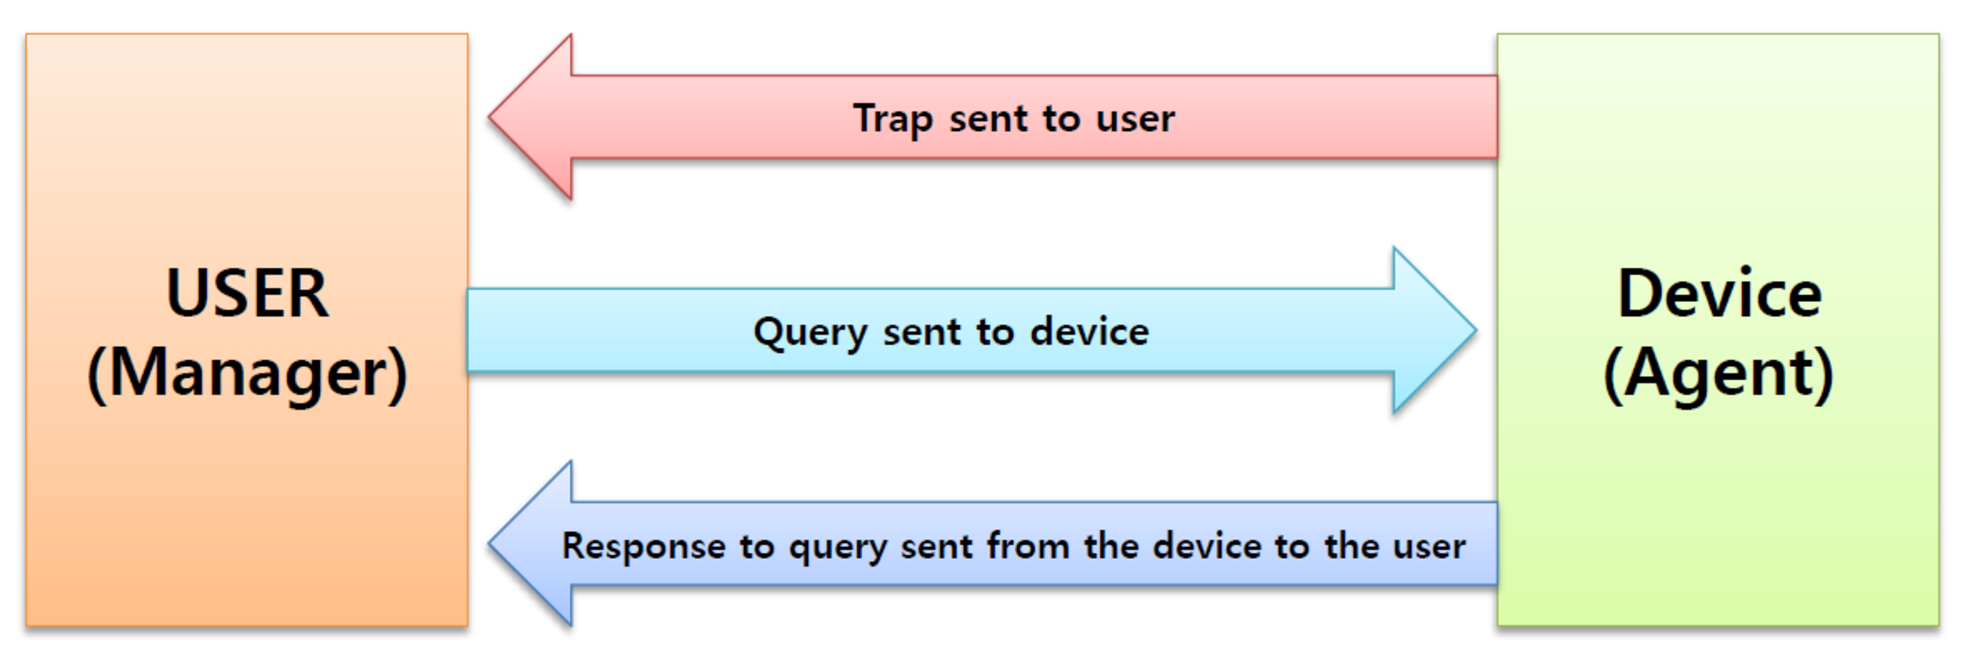
\includegraphics[width=0.65\textwidth]{./images/relationship_m_a.eps}
  \caption{Manager와 Agent의 관계}
  \label{fig:relationship_m_a}   
\end{figure}

\hfill

\section{EPICS}
EPICS (Experimental Physics and Industrial Control System)는 Los Alamo은 국립 연구소와 Argonne 국립 연구소에서 공동개발 되어 오픈 라이센스로 제공되는 실시간 분산 제어 시스템으로 네트워크로 연결된 다양한 장비들의 모니터링 및 제어를 위해 사용된다. EPICS는 현재 전 세계 과학시설의 개발자들에 의해 개발이 진행되고 있다. EPICS는 그림 \ref{fig:ca}의 EPICS 로고와 같이 네트워크 기반의 클라이언트/서버 구조이며, TCP/UDP 프로토콜을 사용하는 CA (Channel Access) 통신 프로토콜을 사용하여 IOC (Input Output Controllers)를 통해 PV (Process Variable)를 주고받는다. 클라이언트는 PV에 접근하며, 서버는 PV에 대한 접근을 제공한다. 특히, CA는 높은 대역폭, soft real-time networking 제어가 요구되는 응용프로그램들에 맞춰 설계되었고, 이는 엄청난 수의 컴퓨터와 장비들을 포함한 제어시스템 구축에 EPICS가 사용될 수 있는 이유이다. 또한, EPICS는 신뢰성 레벨을 제공하며, 이미 구축된 시스템의 유지보수가 쉽다는 장점이 있다\citep{epics}. 

\begin{figure}[h!]
  \centering
  
\includegraphics[width=0.3\textwidth]{./images/epics.eps}
  \caption{Channel Access 구조}
  \label{fig:ca}     
\end{figure}

\section{EPICS와 SNMP의 통합}
EPICS와 통합된 네트워크 기반의 제어 시스템 구축에 SNMP가 용이한 이유는 가속기 제어 시스템에 사용될 장비와 장치들은 Ethernet 환경을 통해 연결되며, 대부분 SNMP를 지원하기 때문이다. 따라서 EPICS와 SNMP의 통합은 중이온가속기 중앙 제어 시스템의 일관성, 유지관리의 용이성, 그리고 최적화 기술의 습득 및 축적의 관점에서 중요하다. 그림 \ref{fig:architecture}은 EPICS와 SNMP 통합 시스템의 구조로, 통합 시스템에서 모니터링 및 제어될 장비는 SNMP MIB를 통해 EPICS와 연결되고, 이는 IOC로 개발되어 CA를 통해 PV와 장비를 통신할 수 있게 한다. PV는 MIB가 가진 장비의 정보로 모니터링 및 제어에 사용된다\citep{epicssnmp}. 

\begin{figure}[h!]
  \centering
  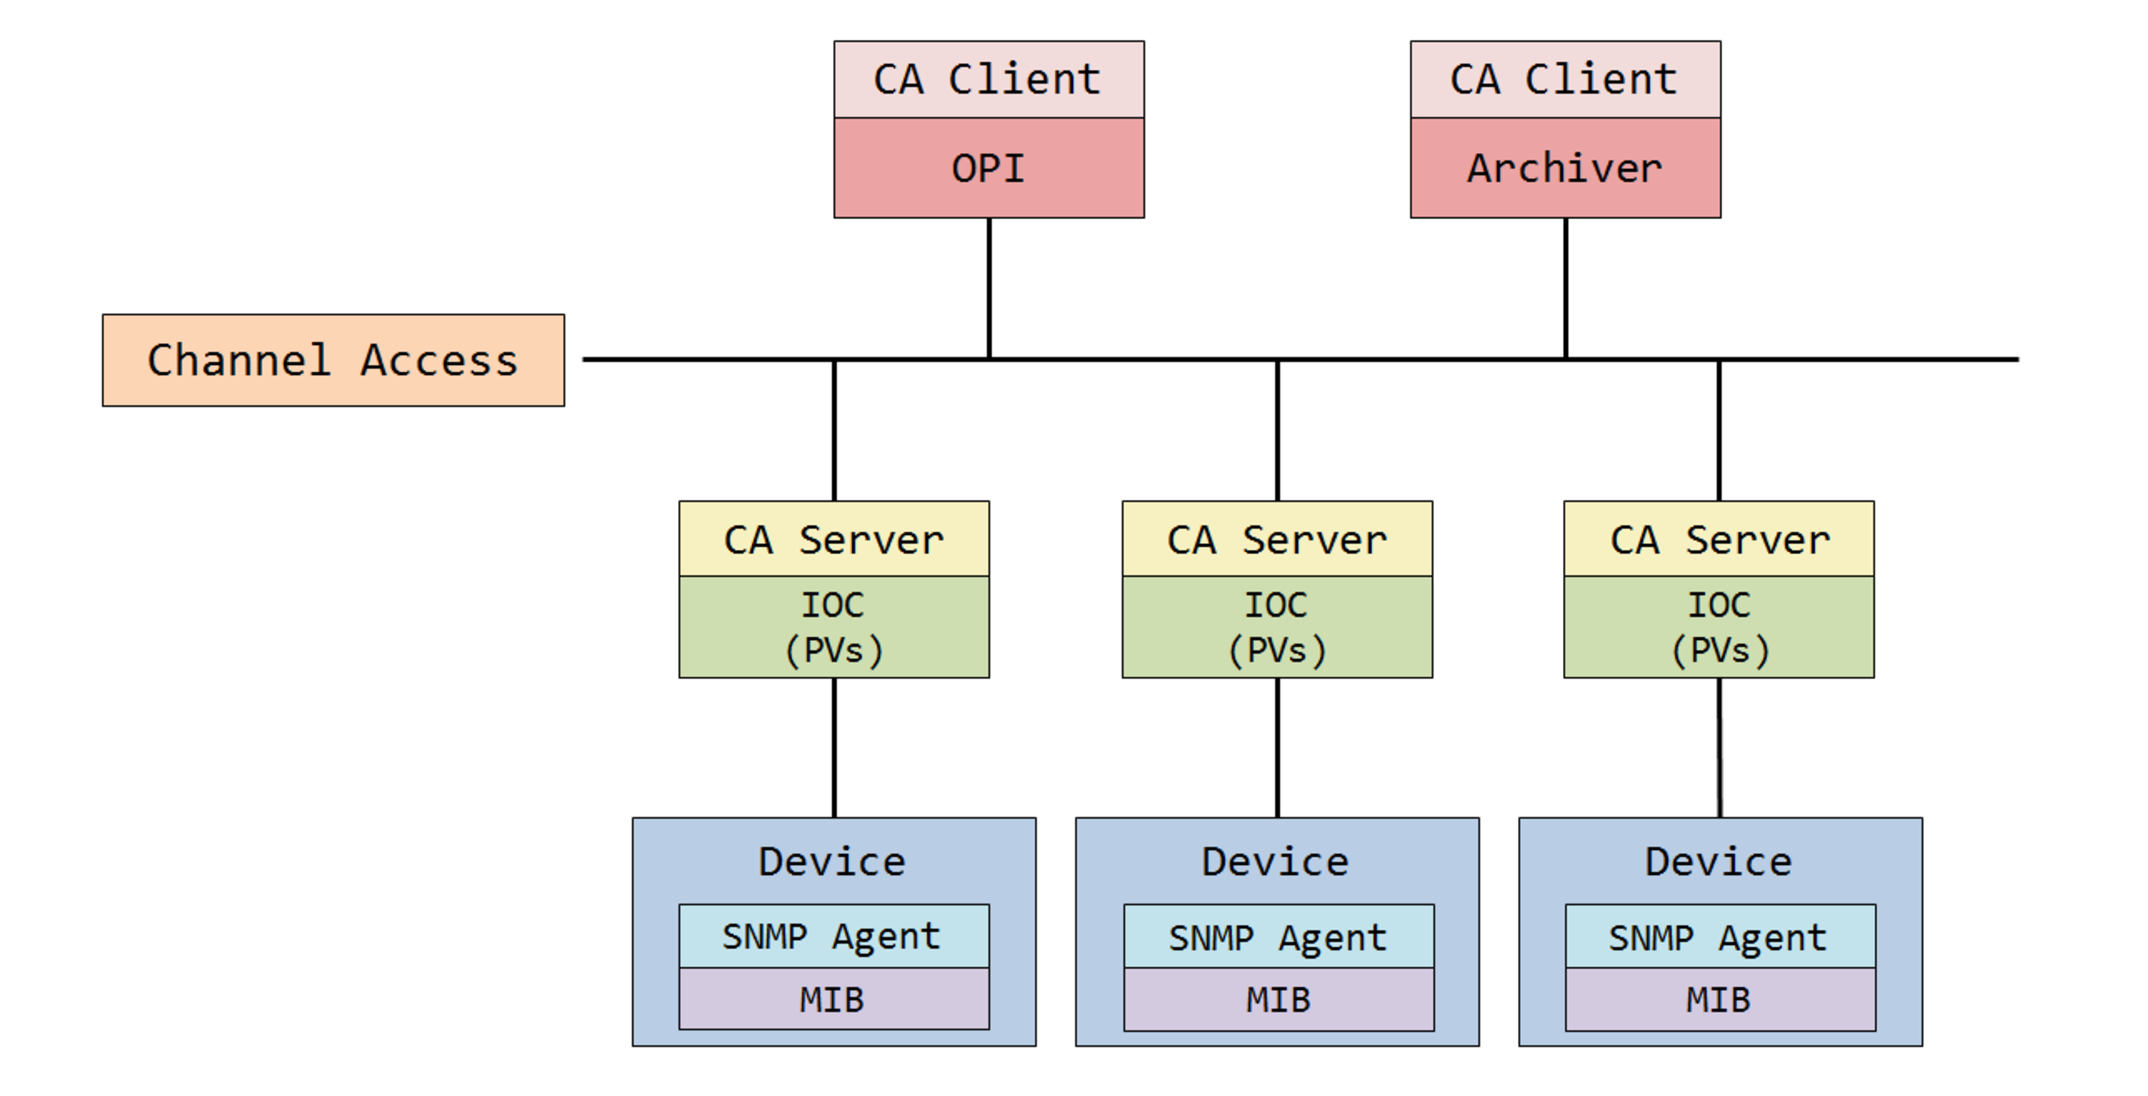
\includegraphics[width=0.89\textwidth]{./images/architecture.eps}
  \caption{EPICS와 SNMP 통합 시스템 아키텍쳐}
  \label{fig:architecture}   
\end{figure}

\chapter{EPICS IOC Support Modules}
EPICS IOC Support Module은 다른 종류의 인터페이스를 가진 하드웨어에 따라 새로운 타입의 레코드나 소프트웨어를 지원하는 Module인 Soft Support와 IOC 내에서 사용 가능한 하드웨어를 지원하는 Module인 Hardware Support로 분류된다. SNMP Soft Support Module은 이미 다수의 개발자에 의해 devSNMP와 이를 보완한 snmp-nscl 등이 존재한다. 본 문서에서는 NSCL/FRIB의 SNMP Device Support Module(snmp-nscl)을 사용하여 초기 버전의 모니터링 시스템을 구축한다\citep{modules}.

\section{NSCL/FRIB SNMP Device Support Module}
NSCL/FRIB SNMP Device Support Module (이하 snmp-nscl)은 EPICS와 SNMP를 통한 하드웨어 장비와의 통신을 위해 2004년 LANL\footnote{* Los Alamos National Laboratory}의 Richard Dubney에 의해 최초 개발된 후 DESY\footnote{* Deutsches Elektronen-Synchrotron}의 Albert Kagarmanov에 의해 개발된 devSNMP를 기반으로 NSCL\footnote{* National Superconducting Cyclotron Laboratory}/FRIB\footnote{* Facility for Rare Isotope Beams}의 John Priller에 의해 개발되었다. DESY의 devSNMP는 snmpv1/2c와 Read만을 지원했다. 이에 devSNMP 코드를 기반으로 snmpv1/2c/3과 Read/ Write를 지원하는 snmp-nscl이 개발되었고, 이는 현재 Wiener/ISEG/MPOD power supply crates에 초점을 두고 RC9 버전까지 개발되었으며, SNMPv2에 최적화 되어있다\citep{devsnmp}. 

\subsection{사용 방법}
snmp-nscl을 사용하여 SNMP를 통해 하드웨어와 EPICS가 통신하기 위해서는 Net-SNMP library와 SNMP를 지원하는 장비, 그리고 장비의 MIB파일이 필요하다. MIB는 보통 리눅스 시스템에서 아래의 경로에 있다.

\begin{lstlisting}[style=termstyle]
/usr/local/share/snmp/mibs/ 
/usr/share/mibs
\end{lstlisting}

하지만 일반적인 경로에 없을 경우, 아래와 같이 IOC st.cmd에 epics환경변수로 MIB의 경로를 추가할 수 있다.

\begin{lstlisting}[style=termstyle]
epicsEnvSet("MIBDIRS", "+$(TOP)/mibs:/some/other/directory")
\end{lstlisting}

기본적인 설정을 끝낸 후, 장비를 모니터링 및 제어하기 위해서는 원하는 정보 값 즉, MIB의 OID 객체를 Support Module의 DB 파일에 record로 정의하여야 한다. snmp-nscl은 SNMP Read/Write에 따라 Input(ai, longin, stringin, waveform(DBF\_STRING, DBF\_CHAR, DBF\_UCHAR))과 Output(ao, longout, stringout)의 record 타입을 지원한다. record는 설명, 디바이스 타입, 스캔 시간, 초기화 등의 다양한 필드\footnote{* 각 레코드 및 필드에 대한 정의는 EPICS Record Reference Manual\citep{record}을 참조 바란다}를 가지며, 필드는 각 Record의 목적에 맞게 사용하면 된다. record의 포맷은 다음과 같다. 

\clearpage

\begin{lstlisting}[style=termstyle]
record(record type, "PV Name") {
 field(DESC, "Description")
 field(DTYP, "Device Type")
 field(SCAN, "Scan rate")
 field(PREC, "Display Precision")
 field(INP/OUT, "@host community OIDname mask dataLength [set_type[special_flags]]")
 .
 .
 }
\end{lstlisting}

snmp-nscl의 정의된 record에서 INP/OUT 필드는 장비의 hostname, community string, 객체의 이름 등의 형태가 snmpget 명령어와 유사하다는 것을 알 수 있다. 

\begin{lstlisting}[style=termstyle]
snmpget -v 2c -c public localhost RFC1213-MIB::sysName.0
\end{lstlisting}

또한, 데이터 타입에 따라 정의되는 mask와 snmpset 명령어의 데이터 타입과 유사하게 set\_type을 정의하여야 한다\footnote{* 추가적인 설명은 devSNMP Documentation\citep{devsnmp}을 참조 바란다}. 예를 들어, 장비의 Voltage 모니터링 및 제어 시 record는 다음과 같다.

\begin{lstlisting}[style=termstyle]
   record(ai, "VoltageRead") {
     field(DESC, "SNMP channel")
     field(DTYP, "Snmp")
     field(SCAN, ".2 second")
     field(PREC, "3")
     field(INP, "@host community WIENER-CRATE-MIB::outputMeasurementSenseVoltage.u0 Float: 100")
   }

   record(ao, "VoltageSet") {
     field(DESC, "SNMP channel")
     field(DTYP, "Snmp")
     field(SCAN, "Passive")
     field(PREC, "3")
     field(OUT, "@host community WIENER-CRATE-MIB::outputVoltage.u0 Float: 100 F")
   }
\end{lstlisting}

각 record는 객체의 Access 권한과 데이터 타입에 따라 VoltageRead, VoltageSet의 이름으로 DB 파일에 정의되고, 이는 PV가 되어 CA를 통한 EPICS와 하드웨어의 통신이 가능해지므로, Voltage 값 변경 및 모니터링을 할 수 있다.

\subsection{장단점}

snmp-nscl은 오랜 개발로 IOC의 안정성이 검증되어있으며, 여러 종류의 IOC Shell Commands가 제공되어 모듈 파라미터 구성과 문제를 진단하는 데 도움이 된다. 또한, SNMP의 다양한 데이터 타입(Integer, String, Gauge, IPAddress 등)을 지원한다. 하지만 v3를 지원한다고는 하나 사용할 수 없으며, 데이터 타입에 따라 mask와 data length 값을 설정해야 하며, 가끔 반환되는 데이터 값이 실제 값과 차이 나는 문제점이 있다.

\clearpage

\section{Device Support Module을 이용한 통합 시스템 구축}
본 문서에서는 SNMPv1/2c를 지원하는 snmp-nscl RC8 버전을 사용하여 중이온가속기 제어 시스템 개발 환경에 맞춘 통합 모니터링 시스템 초기 버전을 구축하였다. 구축된 통합 시스템은 가속기 제어 시스템에 사용되는 다양한 장비 적용에 앞서 사무실 내의 프린터기에 적용되었다. 프린터 모니터링 시스템 구축에 사용된 소프트웨어와 하드웨어는 다음과 같다.

\begin{itemize}
\item Debian Linux 7 Wheezy
\item NET-SNMP v5.4.3
\item EPICS v3.14.12.4
\item snmp-nscl (FRIB SNMP Device Support Module) RC8
\item EPICS CSS (Control System Studio)
\item Printers (XEROX ApeosPort-IV C3375, KYOCERA FS-9530DN)
\end{itemize}

\subsection{Customize 이유 및 수정 사항}
중이온가속기 제어 시스템의 개발 환경은 각 시스템의 원활한 개발 및 개발자 간의 의사소통, 그리고 개발되는 코드들의 단계별 형상관리를 위해 그림 \ref{fig:epicstree}와 같이 표준화된 구조로 되어있다\citep{epicsev}. 따라서 snmp-nscl을 제어 개발 환경과 프린터 모니터링 환경에 최적화하기 위해 아래 몇 가지 사항을 수정하였다.

\begin{figure}[h!]
  \centering
  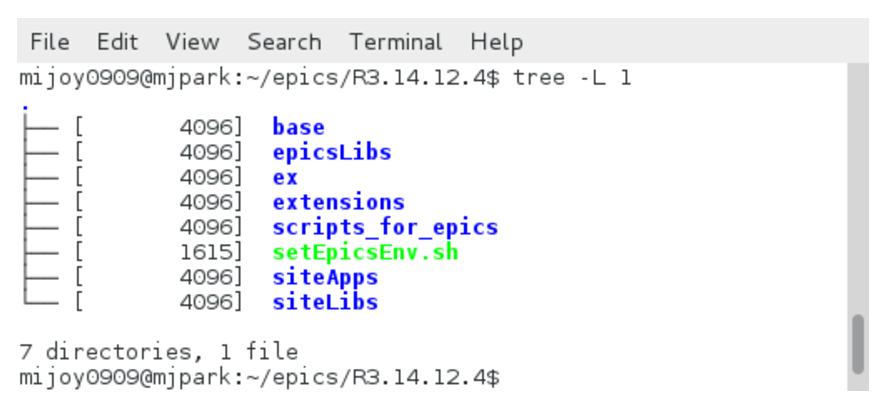
\includegraphics[width=0.89\textwidth]{./images/epicstree.eps}
  \caption{표준화된 중이온가속기 제어 환경의 구조}
  \label{fig:epicstree}   
\end{figure}

\clearpage

\begin{enumerate}
\item 표준화된 중이온가속기 제어 환경에 맞춰 Library (siteLibs)와 Application (siteApps)으로 분리\\
- 중이온가속기 제어 환경은 소프트웨어의 재사용을 위해 Library와 IOC를 개발하는 Application을 분리했다. 따라서 그림 \ref{fig:fribtree}와 같이 Library와 Application이 통합된 구조였던 snmp-nscl을 그림 \ref{fig:makesitelib_frib}, \ref{fig:makesiteapp_frib}의 Makefile 수정과 파일 이동의 과정을 거쳐 표준화된 환경에 맞게 siteLibs(그림 \ref{fig:sitelib_frib})과 siteApps(그림 \ref{fig:siteapp_frib})로 분리했다.

\begin{figure}[h!]
  \centering
  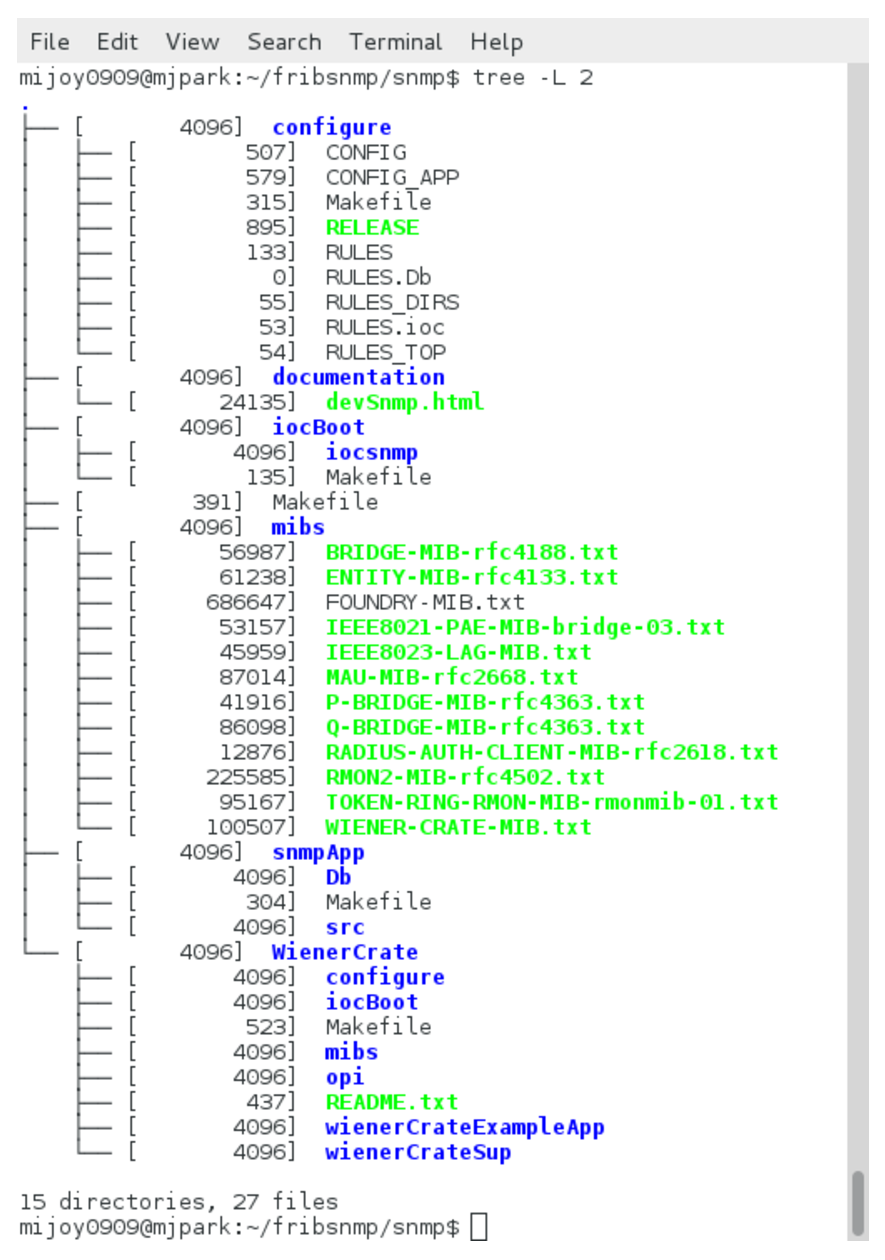
\includegraphics[width=0.7\textwidth]{./images/fribmoduletree.eps}
  \caption{snmp-nscl의 기본 구조}
  \label{fig:fribtree} 
\end{figure}

\clearpage

\begin{figure}[!h]
  \centering
  \subbottom[Labrary Makefile]
  	    {
  	      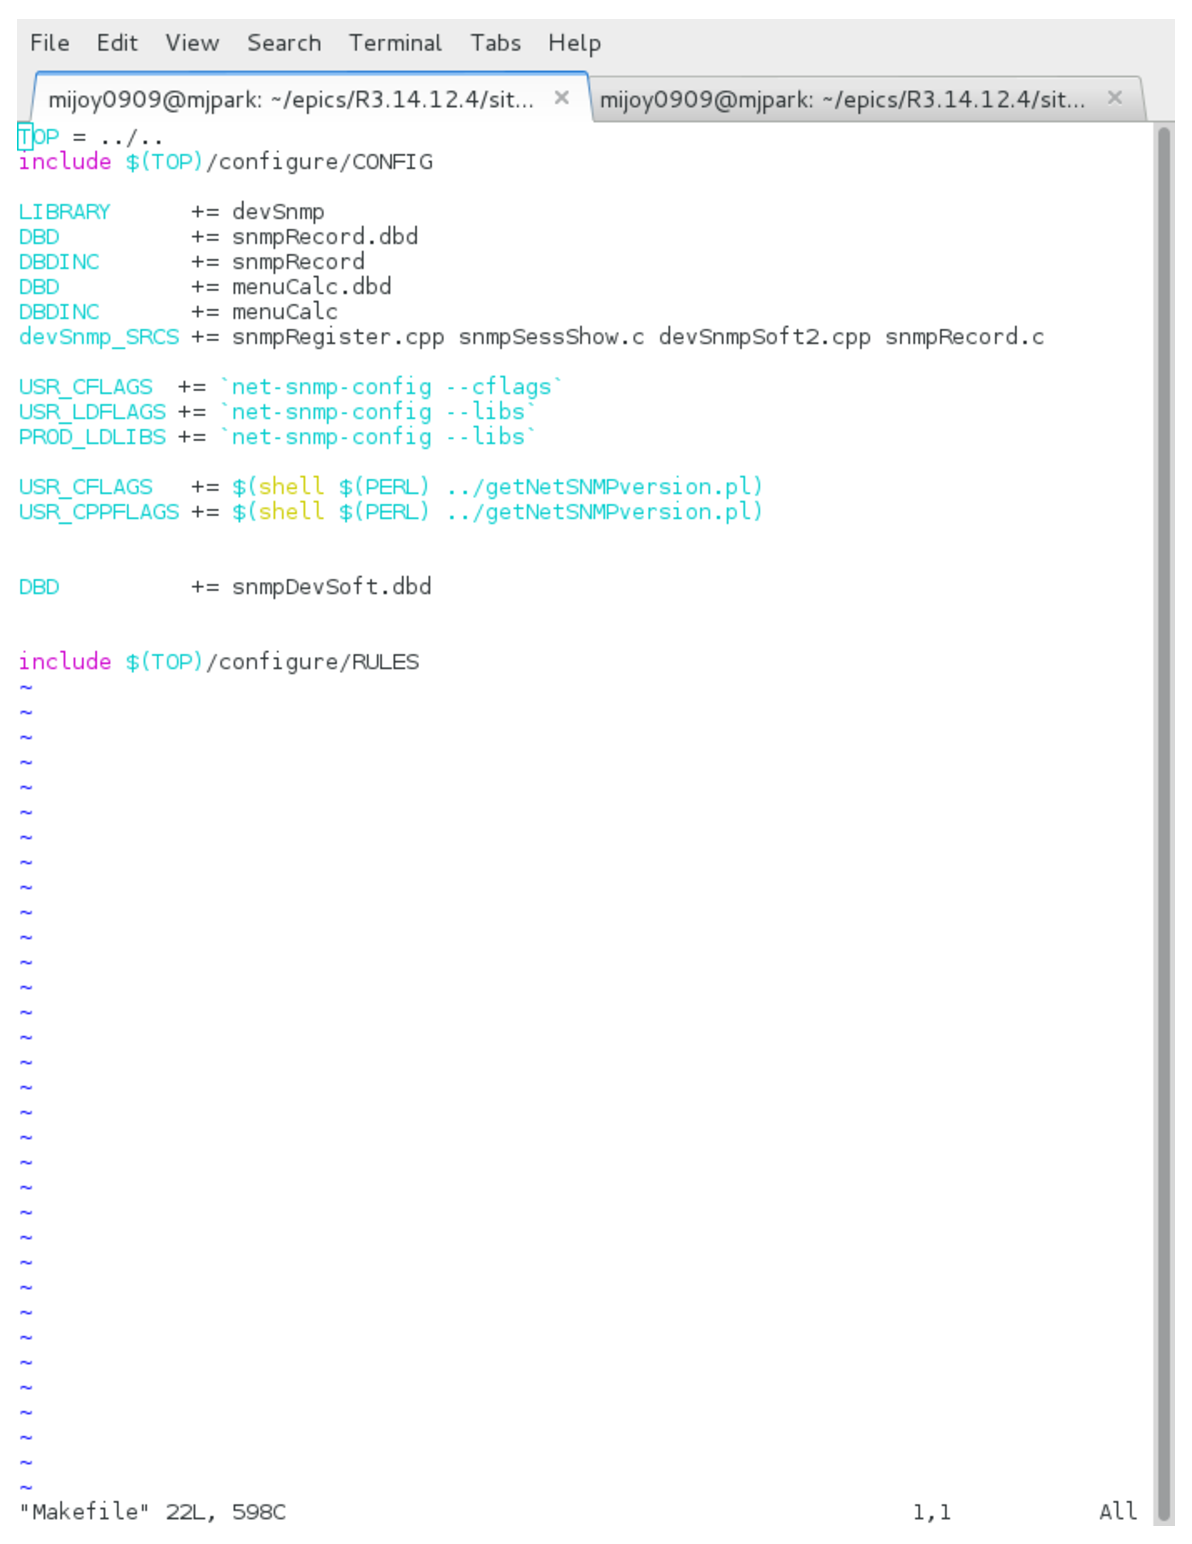
\includegraphics[width=0.45\textwidth]{./images/fribmake_lib.eps}
  	      \label{fig:makesitelib_frib}
  	    }
              \hfill
  \subbottom[Application Makefile]
  	    {
  	      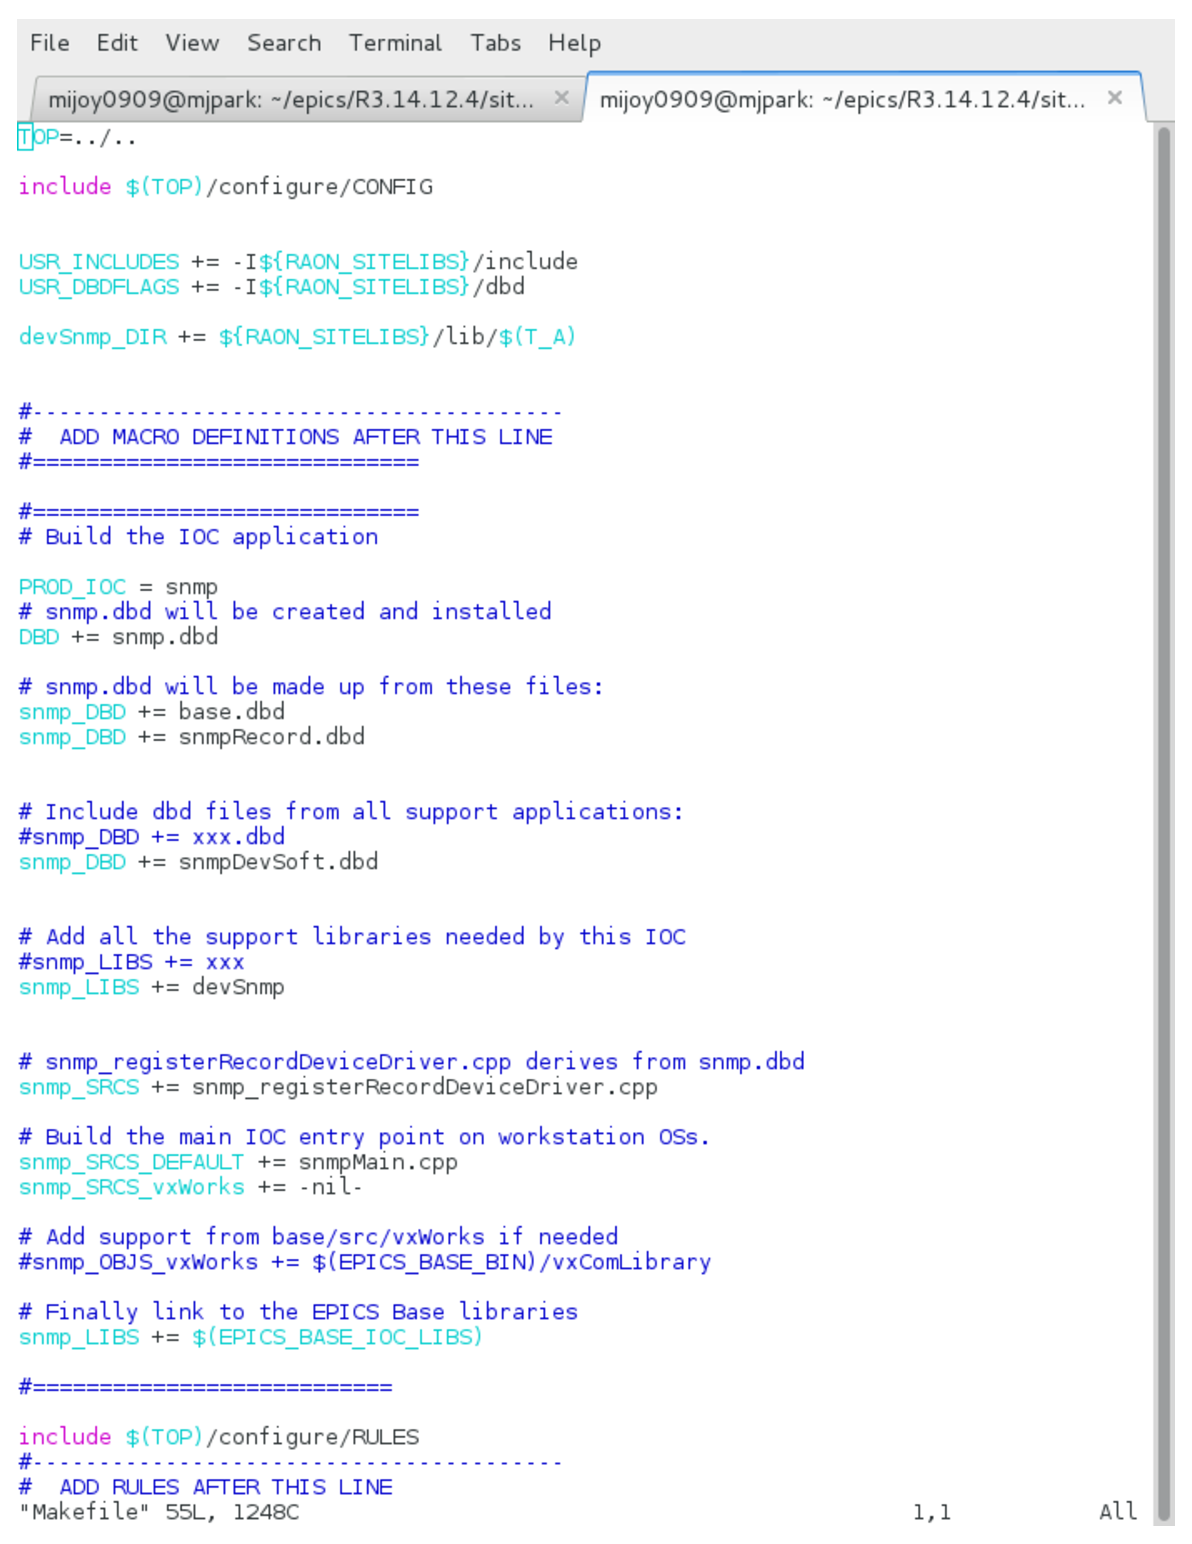
\includegraphics[width=0.45\textwidth]{./images/fribmake_app.eps}
  	      \label{fig:makesiteapp_frib}
  	    }
              \hfill
            
\subbottom[SiteLibs]
	    {
	      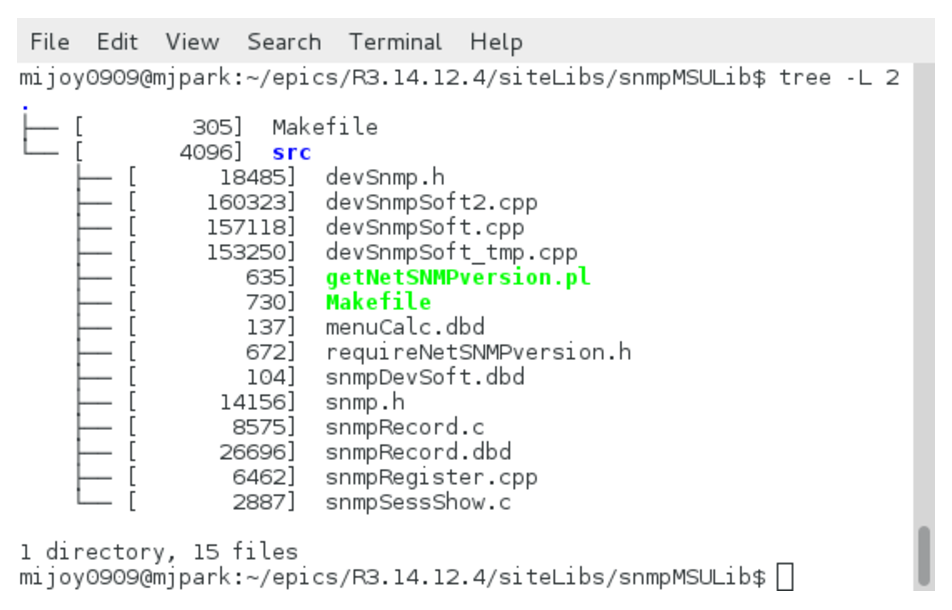
\includegraphics[width=0.45\textwidth]{./images/sitelib_frib.eps}
	      \label{fig:sitelib_frib}
	    }
            \hfill
\subbottom[SiteApps]
	    {
	      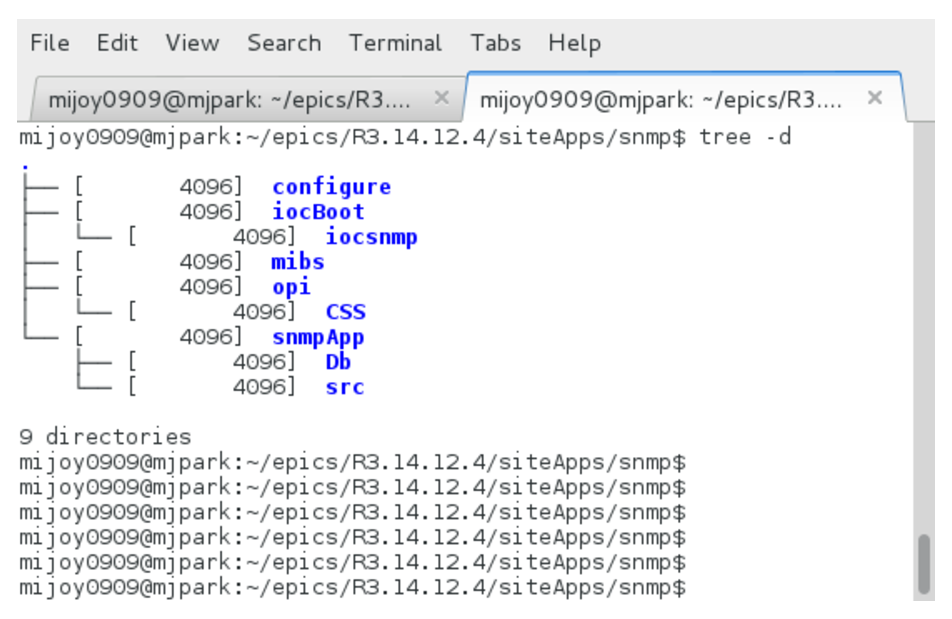
\includegraphics[width=0.45\textwidth]{./images/siteapp_frib.eps}
	      \label{fig:siteapp_frib}
	    }
            \hfill
  \caption
      {
        중이온가속기 제어 개발 환경에 맞춰 수정된 snmp-nscl 
      }
 \label{fig:frib_raon}
\end{figure}

\item snmpRecord, snmpstrRecord 생성\\
- 앞서 언급했듯 snmp-nscl은 SNMP Read/Write에 따라 사용할 수 있는 record를 제공한다. 하지만 본 통합 시스템에서는 기존의 record가 아닌 string타입의 데이터에서 사용될 snmpstrRecord와 그 외 타입의 데이터에서 사용 될 snmpRecord를 생성하여 사용한다. 
 
\begin{lstlisting}[style=termstylenumber]
menu(menuCalc) {
        choice(menu_Plus,"Plus")
        choice(menu_Minus,"Minus")
        choice(menu_Mul,"Multiplication")
        choice(menu_Div,"Division")
}

recordtype(snmp) {
        #include "dbCommon.dbd" 

        field(NAME,DBF_STRING) {
                prompt("Record Name")
                special(SPC_NOMOD)
                size(61)
        }
        field(DESC,DBF_STRING) {
                prompt("Descriptor")
                promptgroup(GUI_COMMON)
                size(41)
        }
        field(MJP,DBF_MENU) {
                prompt("Desired Output")
                promptgroup(GUI_OUTPUT)
                menu(menuCalc)
                interest(1)
        }
.
.
.
}

recordtype(snmpstr) {
        field(NAME,DBF_STRING) {
                prompt("Record Name")
                special(SPC_NOMOD)
                size(61)
        }
        field(DESC,DBF_STRING) {
                prompt("Descriptor")
                promptgroup(GUI_COMMON)
                size(41)
        }
        field(SCAN,DBF_MENU) {
                prompt("Scan Mechanism")
                promptgroup(GUI_SCAN)
                special(SPC_SCAN)
                menu(menuScan)
                interest(1)
        }
.
.
.
}
\end{lstlisting}

Record 생성 후 dbd 파일에 아래와 같이 추가한다. 
\begin{lstlisting}[style=termstyle]
device(snmp,INST_IO,devSnmpSoft,"SoftChannel")
device(snmpstr,INST_IO,devSnmpstrSoft,"SoftChannel")
\end{lstlisting}

\item 소스코드 수정 및 새로운 필드 생성\\
- 프린터의 종이, 잉크의 잔량은 SNMP MIB의 객체에서 전체의 양과 남은 양의 정보를 계산하여 얻을 수 있다. 따라서 snmpRecord 내에 사칙연산 메뉴의 MJP필드를 생성하였으며, siteLibs내 소스코드에 사칙연산을 위한 코드를 추가하였다. 이를 활용하면, 레코드 생성 시 MJP, SVAL, OVAL 필드 사용하여 잔량의 정보를 퍼센트로 나타낼 수 있다.

\begin{lstlisting}[style=termstylenumber]
static long snmpSoftReadback(devSnmp_pv *pPV)
{
  struct snmpRecord *psnmp = (struct snmpRecord *) pPV->record();
  epicsStatus status = epicsError;
  double new_val;
  bool process_record = false;
.
.
.
        psnmp->rval = new_val;
        char oval[40]; 
        char sval[40]; //percent
        switch(psnmp->mjp)
        {
                case menu_Plus: 
                                psnmp->val = ceil(psnmp->rval+psnmp->oval*psnmp->sval);
                break;
                case menu_Minus: 
                                psnmp->val = ceil(psnmp->rval-psnmp->oval*psnmp->sval);
                break;
                case menu_Mul: 
                                psnmp->val = ceil(psnmp->rval*psnmp->oval*psnmp->sval);
                break;
                case menu_Div: 
                                psnmp->val = ceil(psnmp->rval/psnmp->oval*psnmp->sval);
                break;
        }


        process_record = true;
      }
    }
.
.
.
  // process record if needed
  if (process_record) pPV->processRecord();

  return(status);
}
\end{lstlisting}
\end{enumerate}

\subsection{프린터 모니터링 시스템 구축}
그림 \ref{fig:frib_raon}과 같이 수정된 snmp-nscl을 사용하여 프린터 모니터링 시스템을 구축하기 위해서 몇 가지 절차만 수행하면 된다. 

\begin{enumerate}
\item siteLibs에서 snmpMSULib을 컴파일한다.

\begin{lstlisting}[style=termstyle]
mijoy0909@mjpark:~/epics/R3.14.12.4/siteLibs/snmpMSULib$ make
\end{lstlisting}

컴파일 후 그림\ref{fig:libmake}과 같이 siteLis에 dbd, lib, include 폴더가 생기게 되고, 각 폴더에는 아래 리스트의 파일들이 생성된다. 이 파일들은 siteApps에서 IOC 실행에 사용된다.

\begin{lstlisting}[style=termstyle]
# include
mijoy0909@mjpark:~/epics/R3.14.12.4/siteLibs/include$ ls
menuCalc.h  snmpRecord.h

# lib
mijoy0909@mjpark:~/epics/R3.14.12.4/siteLibs/lib/linux-x86_64$ ls
libdevSnmp.a  libdevSnmp.so*


# dbd
mijoy0909@mjpark:~/epics/R3.14.12.4/siteLibs/dbd$ ls
menuCalc.dbd  snmpDevSoft.dbd  snmpRecord.dbd
\end{lstlisting}

\begin{figure}[!h]
  \centering
  \subbottom[Before library Compile]
  	    {
  	      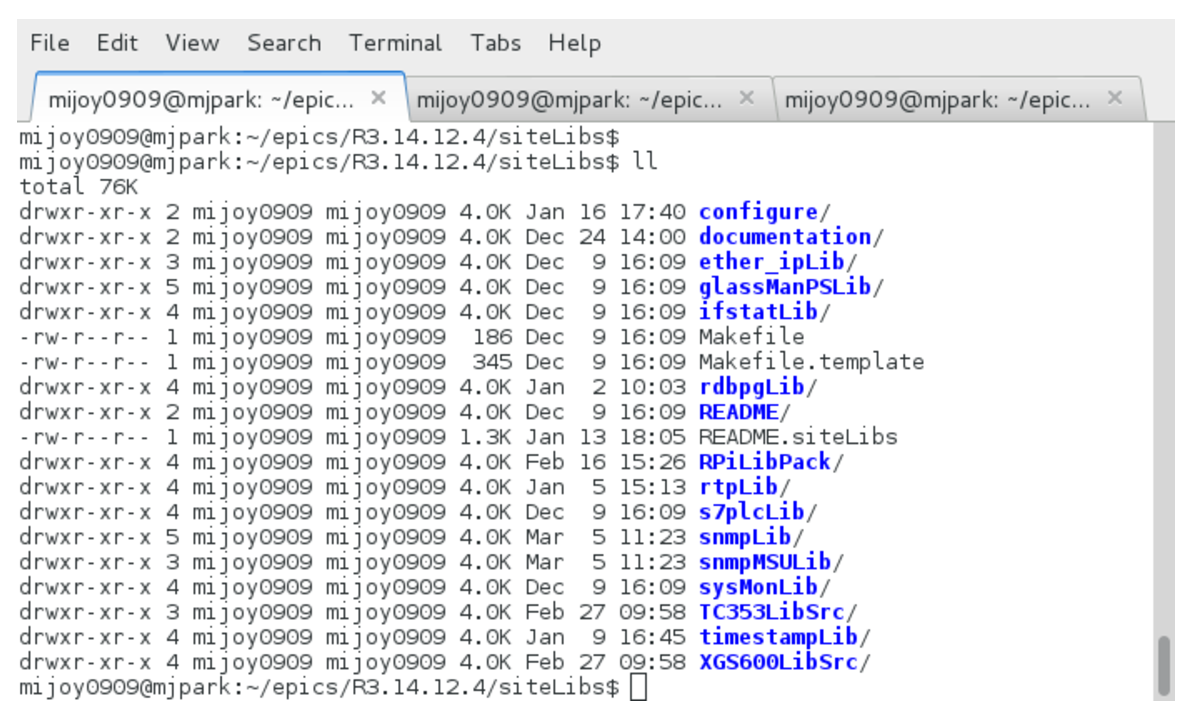
\includegraphics[width=0.45\textwidth]{./images/beforemake_frib2.eps}
  	      \label{fig:beforemake_frib2}
  	    }
              \hfill
  \subbottom[After library Compile]
  	    {
  	      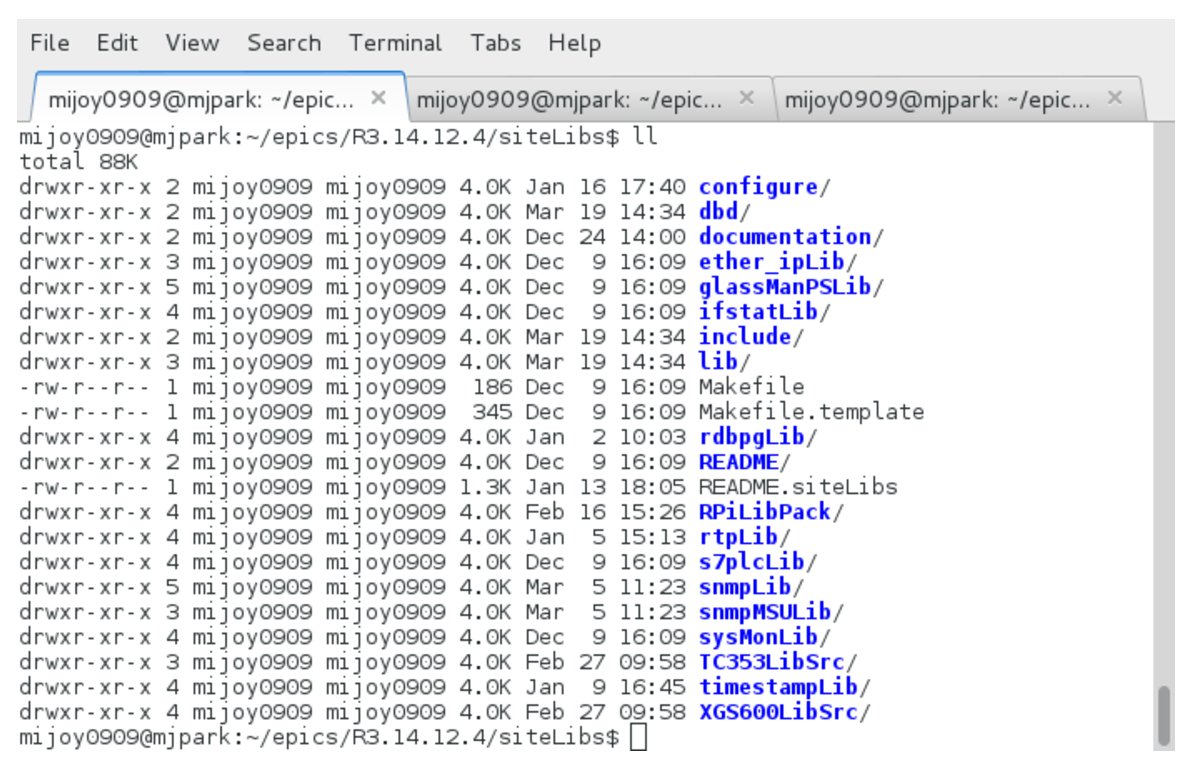
\includegraphics[width=0.45\textwidth]{./images/aftermake_frib2.eps}
  	      \label{fig:aftermake_frib2}
  	    }
              \hfill
            
  \caption
      {
        siteLibs 파일 리스트 
      }
 \label{fig:libmake}
\end{figure}

\item siteApps의 snmpApp/Db에 db 파일을 추가한다.\\
그림 \ref{fig:db}과 같이 모니터링을 원하는 MIB 객체정보를 record에 정의한 db 파일을 만들고, Makefiled에 추가한다.

\begin{figure}[h!]
  \centering
  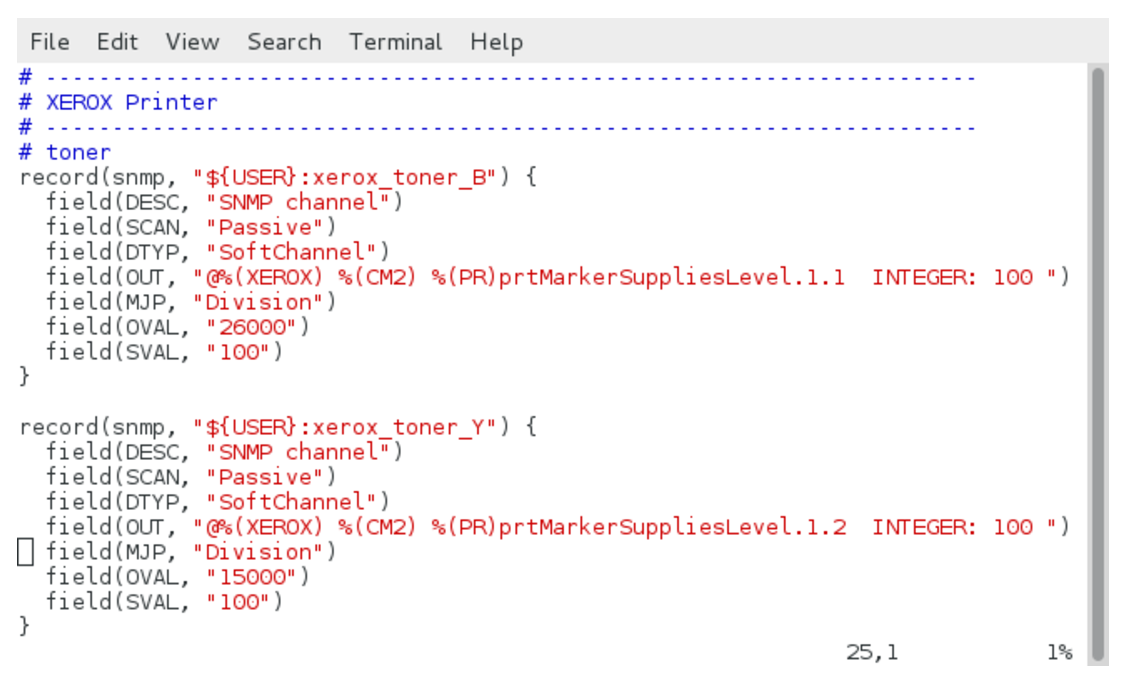
\includegraphics[width=0.5\textwidth]{./images/app.eps}
  \caption{EPICS DB파일}
  \label{fig:db}   
\end{figure}


\begin{lstlisting}[style=termstylenumber]
TOP=../..
include $(TOP)/configure/CONFIG
#----------------------------------------
#  ADD MACRO DEFINITIONS AFTER THIS LINE

#----------------------------------------------------
#  Optimization of db files using dbst (DEFAULT: NO)
#DB_OPT = YES

#----------------------------------------------------
# Create and install (or just install) into <top>/db
# databases, templates, substitutions like this
#DB += xxx.db
DB += printer.vdb

#----------------------------------------------------
# If <anyname>.db template is not named <anyname>*.template add
# <anyname>_template = <templatename>

include $(TOP)/configure/RULES
#----------------------------------------
#  ADD RULES AFTER THIS LINE
\end{lstlisting}

\item siteApps에서 snmp를 컴파일한다.

\begin{lstlisting}[style=termstyle]
mijoy0909@mjpark:~/epics/R3.14.12.4/siteApps/snmp$ make
\end{lstlisting}

컴파일 후 그림 \ref{fig:appmake}와 같이 bin, db, dbd 파일이 생성되고, 각각의 폴더에는 siteLibs과 마찬가지로 IOC 실행에 사용될 파일이 생성된다.

\begin{figure}[!h]
  \centering
  \subbottom[Before Application Compile]
  	    {
  	      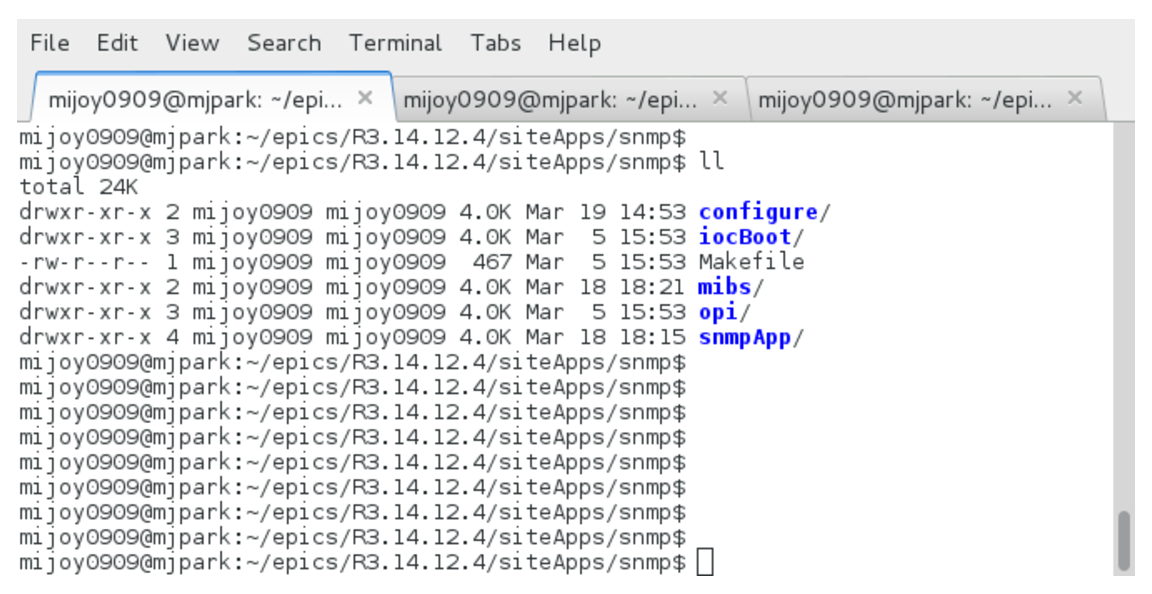
\includegraphics[width=0.45\textwidth]{./images/beforemake_app_frib.eps}
  	      \label{fig:beforemake_frib_app}
  	    }
              \hfill
  \subbottom[After Application Compile]
  	    {
  	      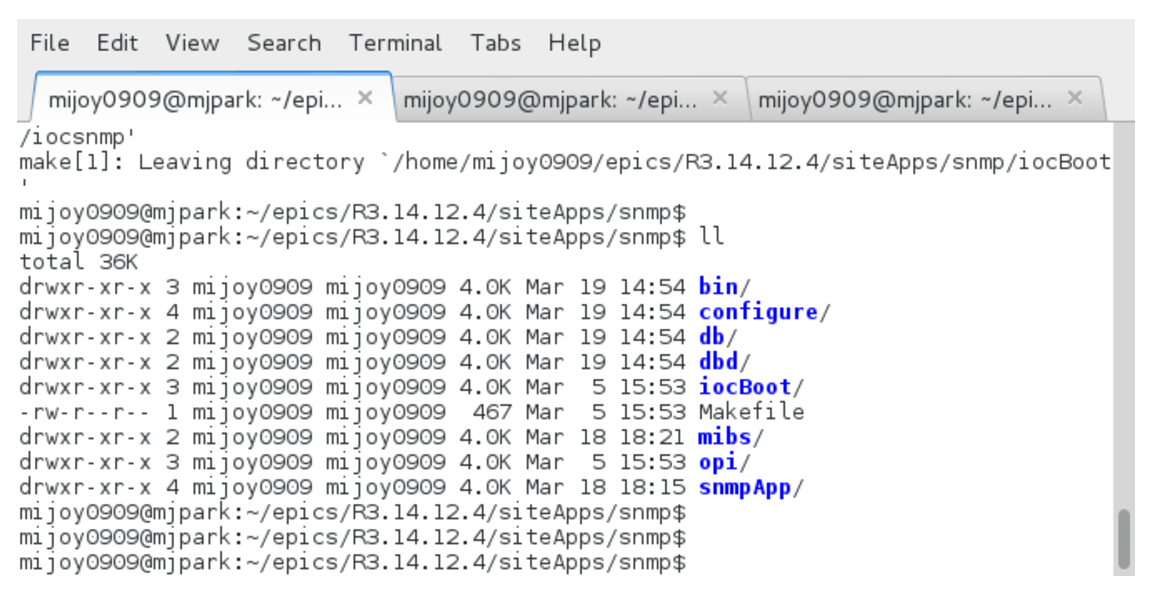
\includegraphics[width=0.45\textwidth]{./images/aftermake_app_frib.eps}
  	      \label{fig:aftermake_frib_app}
  	    }
              \hfill
            
  \caption
      {
        siteApps/snmp 파일 리스트 
      }
 \label{fig:appmake}
\end{figure}

\item IOC 실행 전 st.cmd파일을 수정 및 실행권한을 부여한다.\\
/iocBoot/iocsnmp로 이동 후 st.cmd 파일에 앞서 생성한 db파일을 추가해준다. 이때, MIB파일의 경로, 사용하고자 하는 SNMP의 버전, 사용한 매크로 값에 대한 정보도 추가해준다.

\begin{lstlisting}[style=termstylenumber]
#!../../bin/linux-x86_64/snmp

## You may have to change snmp to something else
## everywhere it appears in this file

< envPaths

cd ${TOP}

epicsEnvSet("MIBDIRS", "+$(TOP)/mibs")
devSnmpSetSnmpVersion("10.1.4.184","SNMP_VERSION_1")
devSnmpSetSnmpVersion("10.1.4.182","SNMP_VERSION_2c")

epicsEnvSet("PR", "Printer-MIB::")
epicsEnvSet("JM", "Job-Monitoring-MIB::")
epicsEnvSet("SMI", "SNMPv2-SMI::")
epicsEnvSet("XM", "XEROX-SERVICE-MONITORING-MIB::")
epicsEnvSet("CM1", "admin")
epicsEnvSet("CM2", "public")
epicsEnvSet("XEROX", "10.1.4.182")
epicsEnvSet("KYOCERA", "10.1.4.184")

## Register all support components
dbLoadDatabase "dbd/snmp.dbd"
snmp_registerRecordDeviceDriver pdbbase

## Load record instances
dbLoadRecords("db/printer.vdb","USER=mijoy0909Host")

cd ${TOP}/iocBoot/${IOC}
iocInit

## Start any sequence programs
#seq sncxxx,"user=mijoy0909Host"
\end{lstlisting}

\begin{lstlisting}[style=termstyle]
mijoy0909@mjpark:~/epics/R3.14.12.4/siteApps/snmp/iocBoot/iocsnmp$ chmod 755 st.cmd
\end{lstlisting}

\item IOC 실행 및 통신 확인 과정을 거친다.\\
IOC가 실행 후 PV 리스트를 확인한 결과는 그림 \ref{fig: printer_ioc}과 같다. 

\begin{figure}[h!]
  \centering
  	      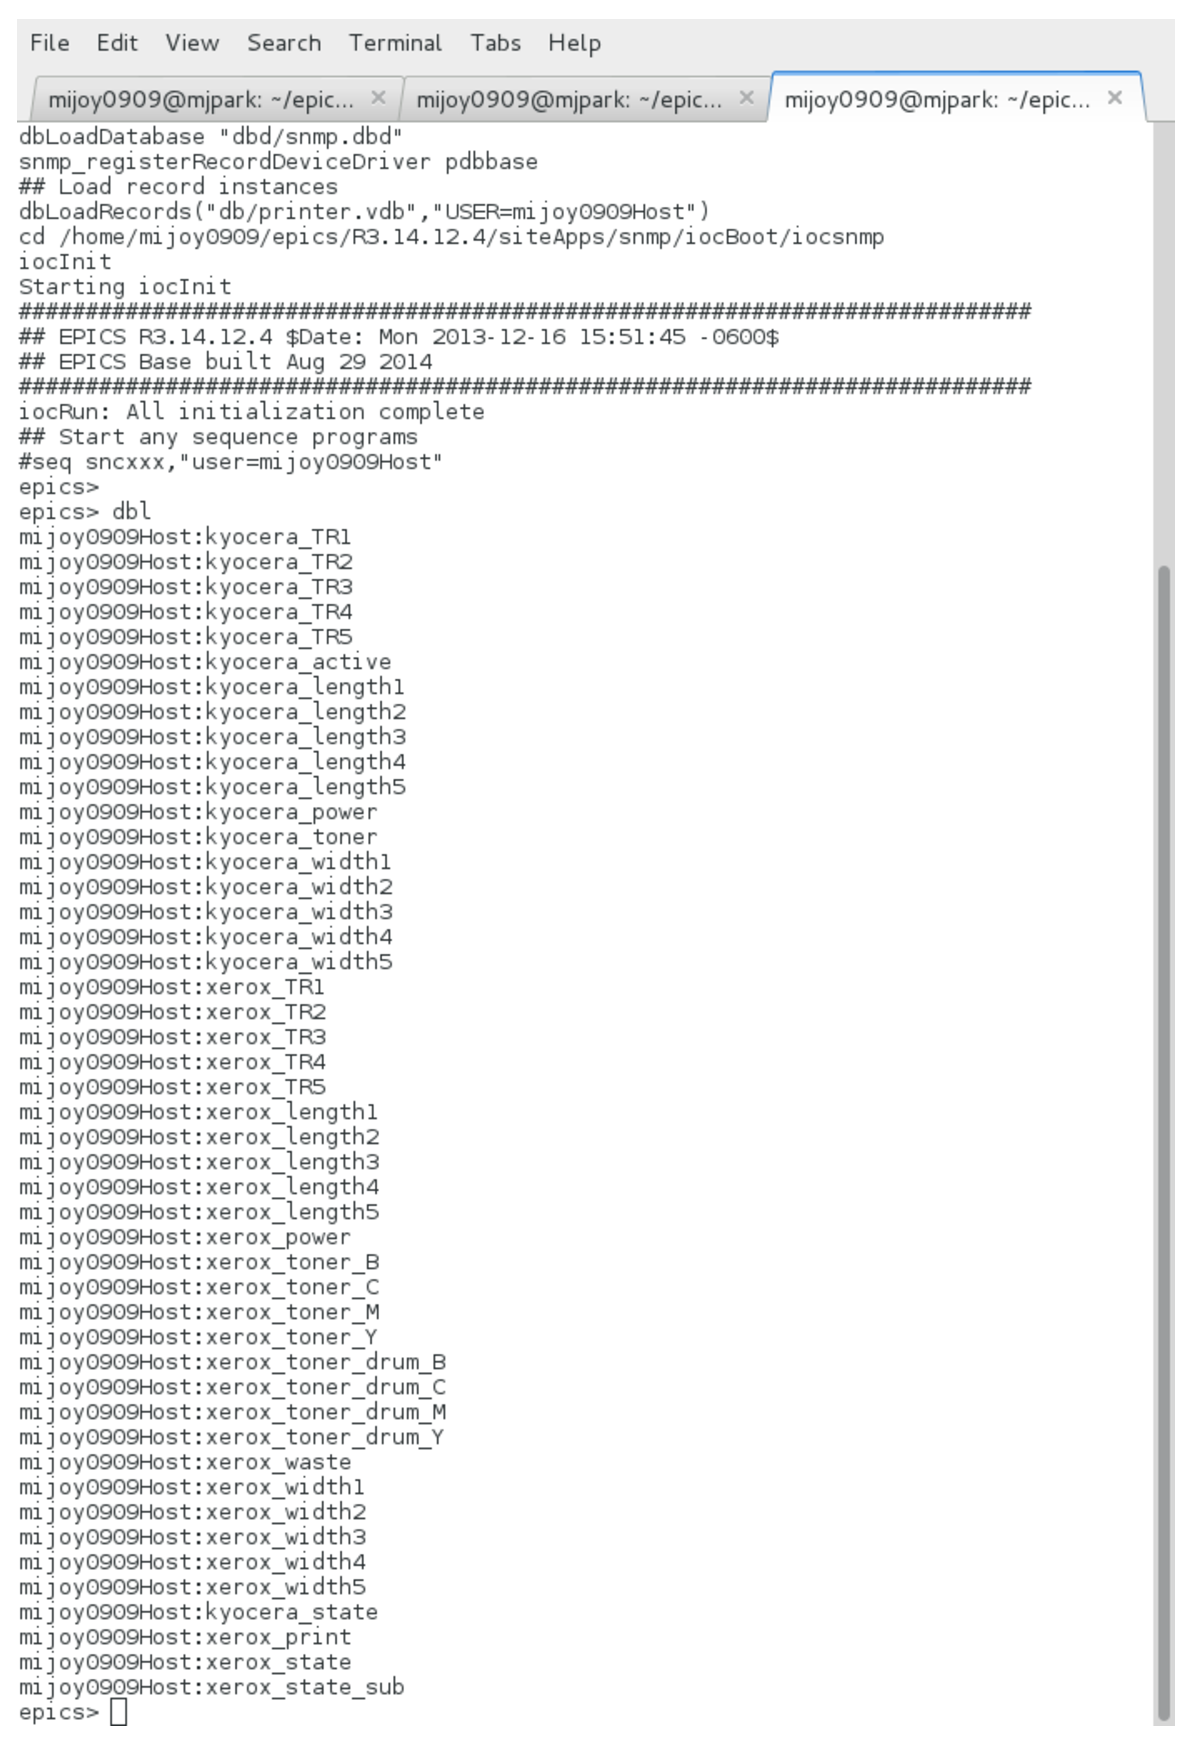
\includegraphics[width=0.5\textwidth]{./images/printer_ioc.eps}
  \caption{EPICS IOC 실행 및 PV 리스트}
  	      \label{fig: printer_ioc}
\end{figure}

PV가 장비와 통신 되고 있는지 확인하기 위해 EPICS의 Command, CA monitor, snmpget을 값을 확인한 결과, 같은 값을 보이므로 EPICS로 프린터기가 모니터링됨을 확인할 수 있다.  
\begin{lstlisting}[style=termstyle]
# EPICS Command
epics> dbpr mijoy0909Host:xerox_state
ASG:                DESC: SNMP channel  DISA: 0             DISP: 0             
DISV: 1             NAME: mijoy0909Host:xerox_state         SEVR: NO_ALARM      
STAT: NO_ALARM      TPRO: 0             VAL: Printing...    
\end{lstlisting}

\begin{lstlisting}[style=termstyle]
# CA monitor
mijoy0909@mjpark:~$ camonitor mijoy0909Host:xerox_state
mijoy0909Host:xerox_state      2015-03-19 15:23:32.007583 Printing...  
\end{lstlisting}

\begin{lstlisting}[style=termstyle]
# snmpget
mijoy0909@mjpark:~$ snmpget -v 2c -c public 10.1.4.182 prtConsoleDisplayBufferText.1.1
Printer-MIB::prtConsoleDisplayBufferText.1.1 = STRING: "Printing..."
\end{lstlisting}

\end{enumerate}

\subsection{OPI 구현}
IOC가 실행되어 각각의 PV들이 CA 통신으로 프린터기의 정보를 모니터링하면, EPICS의 UI (User Interface) 프로그램인 CSS (Control System Studio)를 사용하여 프린터 모니터링 시스템의 OPI (Operator Interface)를 구현한다. 그림 \ref{fig:css_monitoring}은 프린터의 상태, 소모품의 잔량 등의 정보 확인 및 종이 걸림, 소모품 부족 등의 알림을 알 수 있도록 구현되었다.

\begin{figure}[h!]
  \centering
  \includegraphics[width=0.8\textwidth]{./images/css_monitoring.eps}
  \caption{프린터 모니터링 시스템 OPI}
  \label{fig:css_monitoring}   
\end{figure}

\clearpage

\chapter{EPICS Integration}
이미 개발되어있는 EPICS Support Module을 사용하여 EPICS와 SNMP를 통합할 수 있지만, 자체적으로 중이온가속기 제어 시스템에 최적화된 통합 시스템 구축을 위해 유동적이고, API 확장이 가능한 Net-SNMP와 EPICS를 통합한다. 통합 시스템은 모니터링 시에는 SNMPv2c, 제어 시에는 SNMPv3로 최적화한다.

\section{Legacy SNMP Code (Net-snmp tutorial)}
Net-SNMP는 1992년 Carnegie Mellon University에서 시작된 프로젝트에서 개발된 공개코드 SNMP(v2.1.2.1)를 기반으로 개발된 패키지이다. 이는 CMU-SNMP, UCD-SNMP를 거쳐 2000년 Net-SNMP가 되어, IPv4, IPv6를 사용하여 SNMPv1/2c/3을 구현하고, Agent와 Manager가 정보를 주고받을 수 있도록 snmpget, set, walk 등의 명령어를 제공하는 패키지로, Tutorials를 제공해 패키지 사용에 도움을 준다\citep{netsnmp}\citep{tutorials}. 따라서 Net-SNMP에서 제공하는 Client/Mananger Coding Tutorials를 활용하여 SNMP와 Net-SNMP 명령어와 패키지 등에 대해 이해하고 EPICS와의 통합에 사용한다. 
 
\subsection{Simple Async Application}
Client/Mananger Coding Tutorials에는 장비에서 원하는 정보 값을 얻는 방법으로 동기식의 Simple application와 비동기식의 Simple Async Application이 있다. 
Simple Async Application 예제의 Host, Community, OID 값을 원하는 장비에 맞춰 변경해 컴파일한 후 실행시키면 아래와 같이 Simple application의 결과와 Simple Async Application 결과를 모두 보여준다. 

\begin{lstlisting}[style=termstyle]
mijoy0909@mjpark:~/rawcode$ make asyncapp
gcc -I. `net-snmp-config --cflags`   -c -o asyncapp.o asyncapp.c
gcc -o asyncapp asyncapp.o `net-snmp-config --libs`
\end{lstlisting}

\begin{lstlisting}[style=termstylenumber]
mijoy0909@mjpark:~/rawcode$ ./asyncapp 
---------- synchronous -----------
11:08:18.712241 10.1.4.182: HOST-RESOURCES-MIB::hrDeviceDescr.1 = STRING: FUJI XEROX ApeosPort-IV C3375  v 84. 18.  0 Multifunction System
11:08:18.714129 10.1.4.182: Printer-MIB::prtGeneralPrinterName.1 = STRING: "ApeosPort-IV C3375 "
11:08:18.724114 10.1.4.182: Printer-MIB::prtConsoleDisplayBufferText.1.1 = STRING: "Print-User Action"
11:08:18.760751 10.1.4.184: HOST-RESOURCES-MIB::hrDeviceDescr.1 = STRING: FS-9530DN
11:08:18.780953 10.1.4.184: Printer-MIB::prtGeneralPrinterName.1 = STRING: "FS-9530DN"
11:08:19.144312 10.1.4.184: Printer-MIB::prtConsoleDisplayBufferText.1.1 = STRING: "Please wait     "
---------- asynchronous -----------
11:08:19.185517 10.1.4.182: HOST-RESOURCES-MIB::hrDeviceDescr.1 = STRING: FUJI XEROX ApeosPort-IV C3375  v 84. 18.  0 Multifunction System
11:08:19.185877 10.1.4.184: HOST-RESOURCES-MIB::hrDeviceDescr.1 = STRING: FS-9530DN
11:08:19.186001 10.1.4.182: Printer-MIB::prtGeneralPrinterName.1 = STRING: "ApeosPort-IV C3375 "
11:08:19.186261 10.1.4.184: Printer-MIB::prtGeneralPrinterName.1 = STRING: "FS-9530DN"
11:08:19.194116 10.1.4.182: Printer-MIB::prtConsoleDisplayBufferText.1.1 = STRING: "Print-User Action"
11:08:19.244038 10.1.4.184: Printer-MIB::prtConsoleDisplayBufferText.1.1 = STRING: "Please wait     "
\end{lstlisting}

Simple application은 Agent에 요청을 보내고 응답이 올 때까지 블럭킹되어 대기상태로 있으므로 중이온가속기 제어 시스템에 사용되는 다양한 장비를 모니터링하기엔 적합하지 않다. 반면에 Simple Async Application은 Agent로부터 요청에 대한 응답이 있을 때 callback 형식으로 호출되어 결과를 출력한다. 따라서 EPICS와 SNMP의 통합에는 비동기식으로 데이터를 전송하는 Simple Async Application 예제를 사용한다.

\section{Library 구성}
Simple Async Application(이하 AsyncApp)과 EPICS의 통합에서 Library는 소스코드, Record파일, dbd파일로 구성된다.

\subsection{Record}
AsyncApp과 EPICS IOC의 통신에 사용할 Record를 생성한다. EPICS의 Example IOC Application에서 xxxRecord.dbd를 사용하여 SNMP의 다양한 데이터 타입 중 analog와 string 타입의 snmpRecord와 snmpstrRecord의 dbd파일을 생성한다. 이때, 기본적인 필드 외에 그림 \ref{fig:recorddbd}와 같이 통신에 필요한 장비의 Host, Community string, OID와 snmp버전 정보 및 인증과 암호화 비밀번호에 대한 필드를 추가한다.

\begin{figure}[h!]
  \centering
  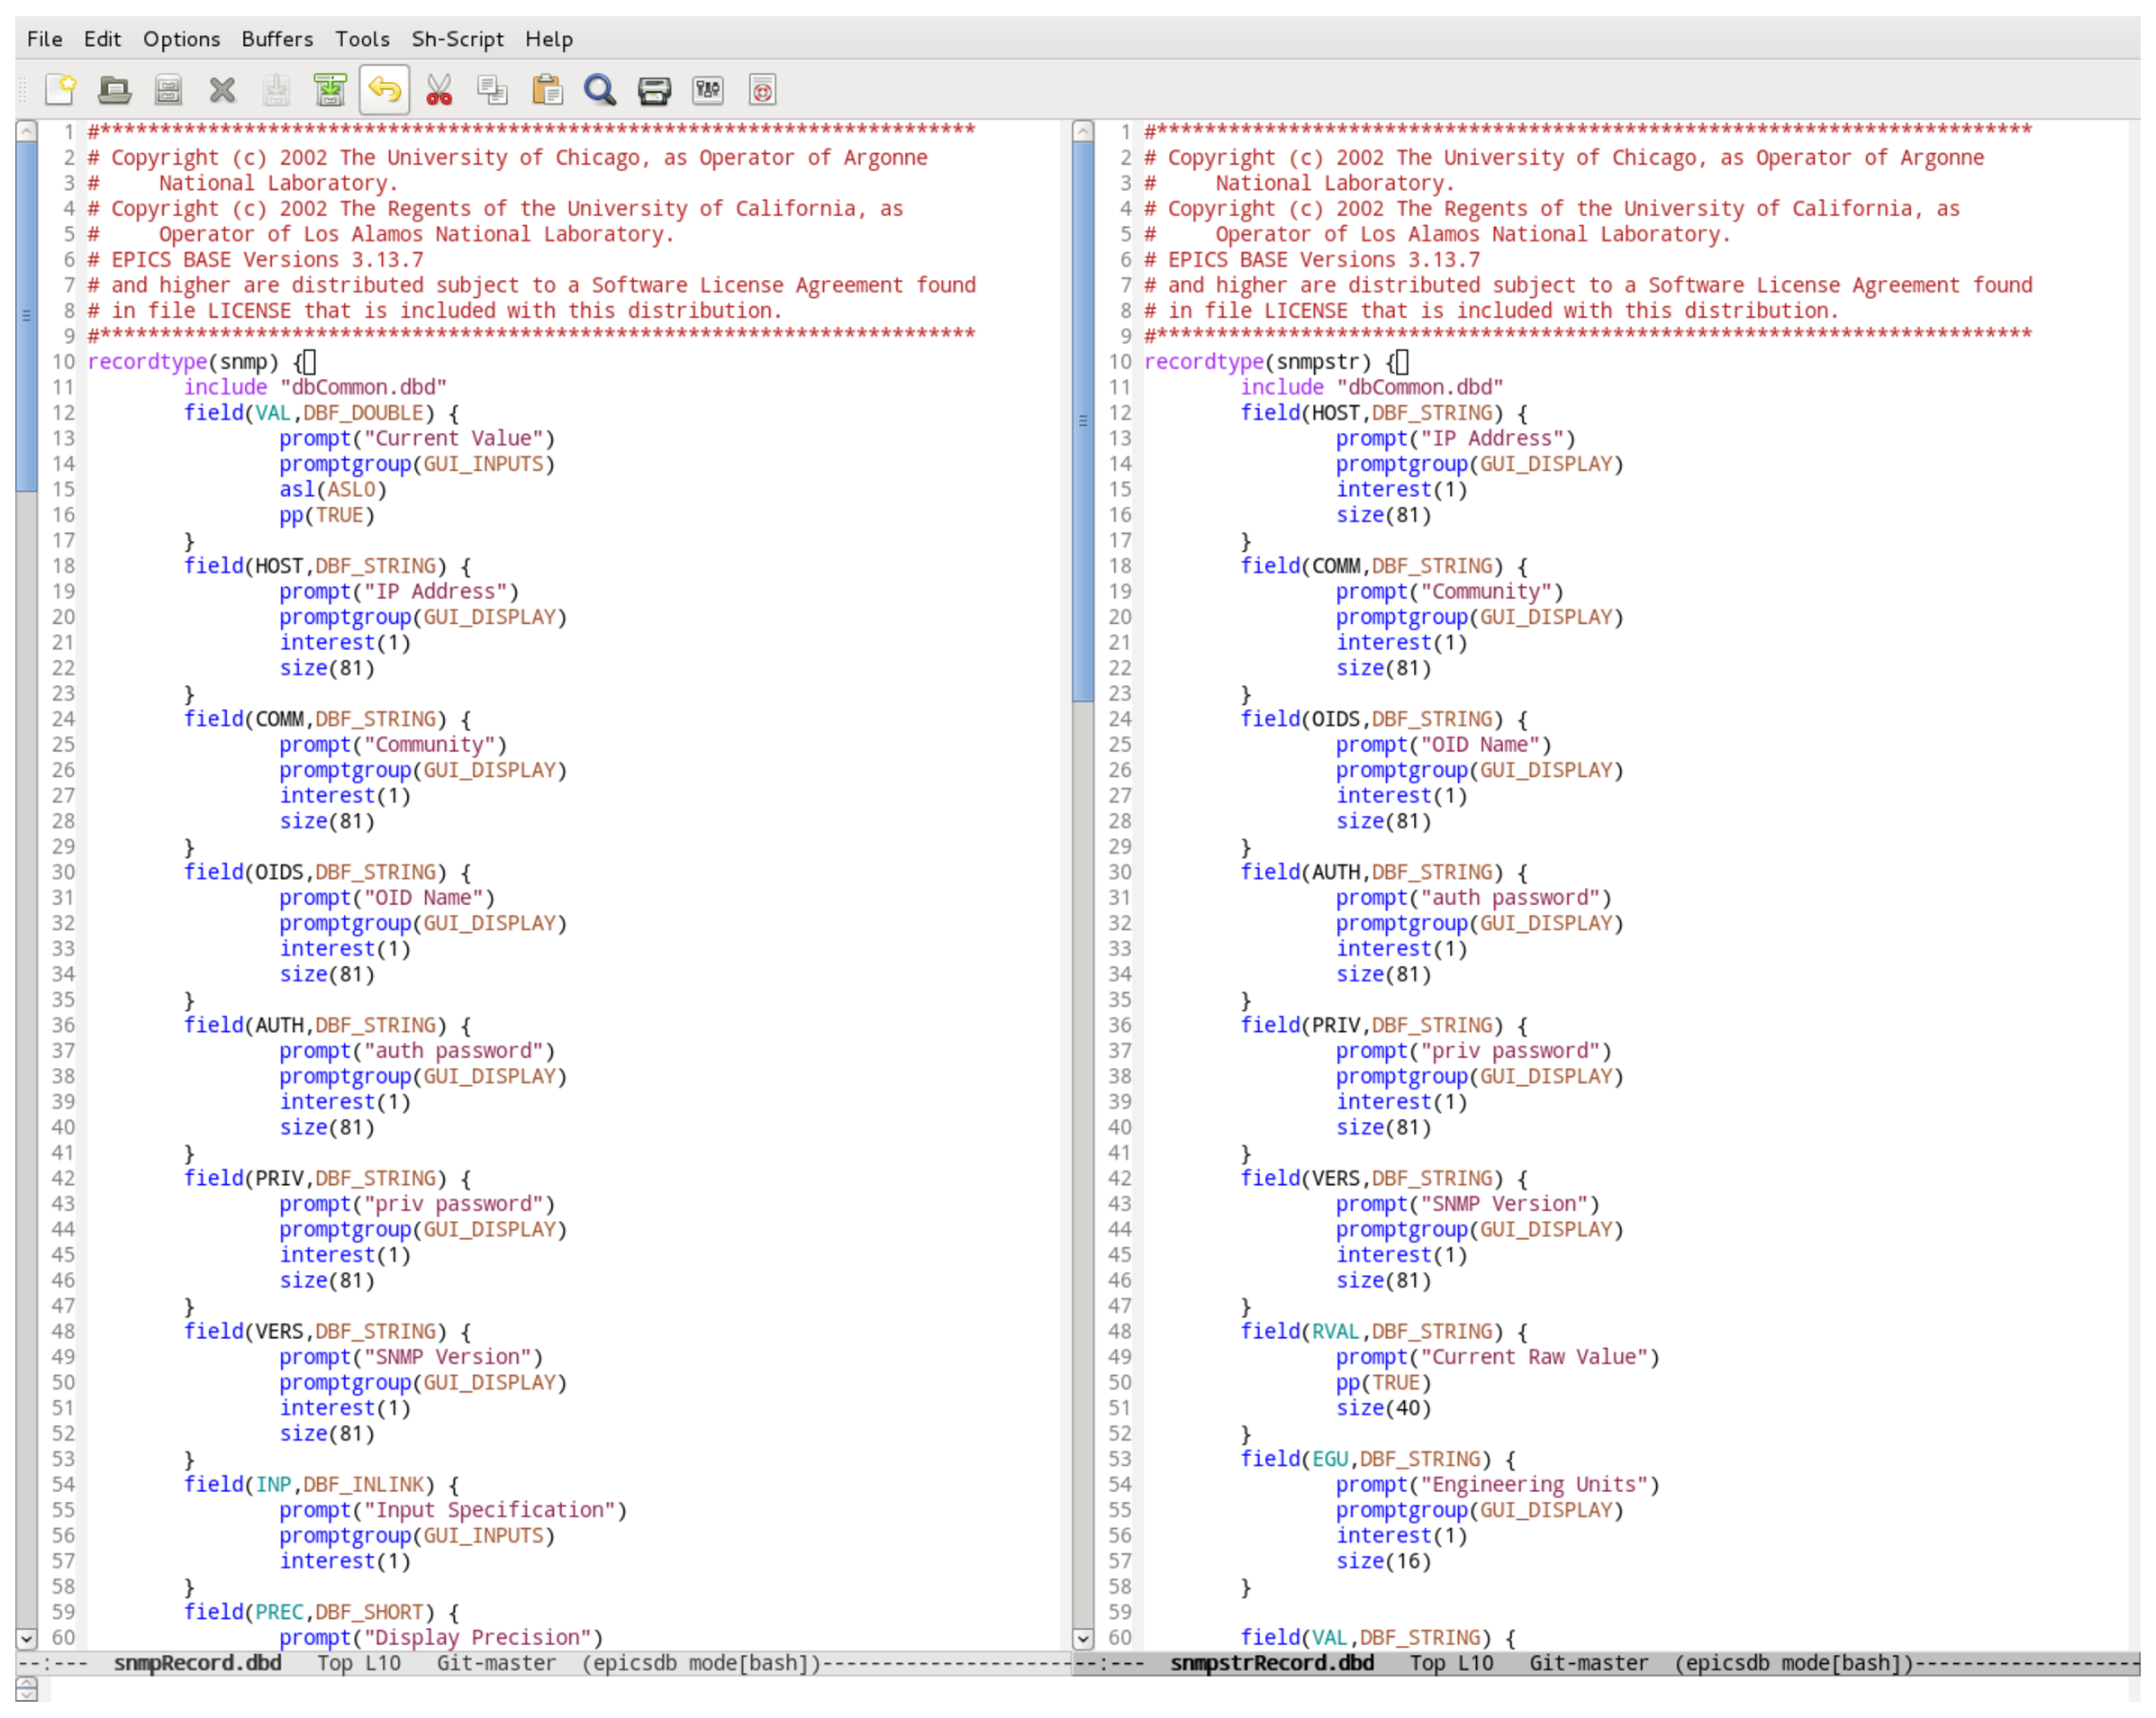
\includegraphics[width=0.89\textwidth]{./images/recorddbd.eps}
  \caption{record.dbd 파일 (left: snmpReocrd.dbd right: snmpstrRecord.dbd)}
  \label{fig:recorddbd}   
\end{figure}

Record 생성 후 xxxRecord.c를 수정하여 그림 \ref{fig:recordc}과 같이 snmpRecord.c와 snmpstrRecord.c를 생성한다. 이때 string 타입의 레코드는 analog타입의 레코드와 달리 알람을 설정 할 필요가 없으므로 snmpstrRecord.c는 process함수의 checkAlarms부분을 주석처리 한다. 

\begin{figure}[h!]
  \centering
  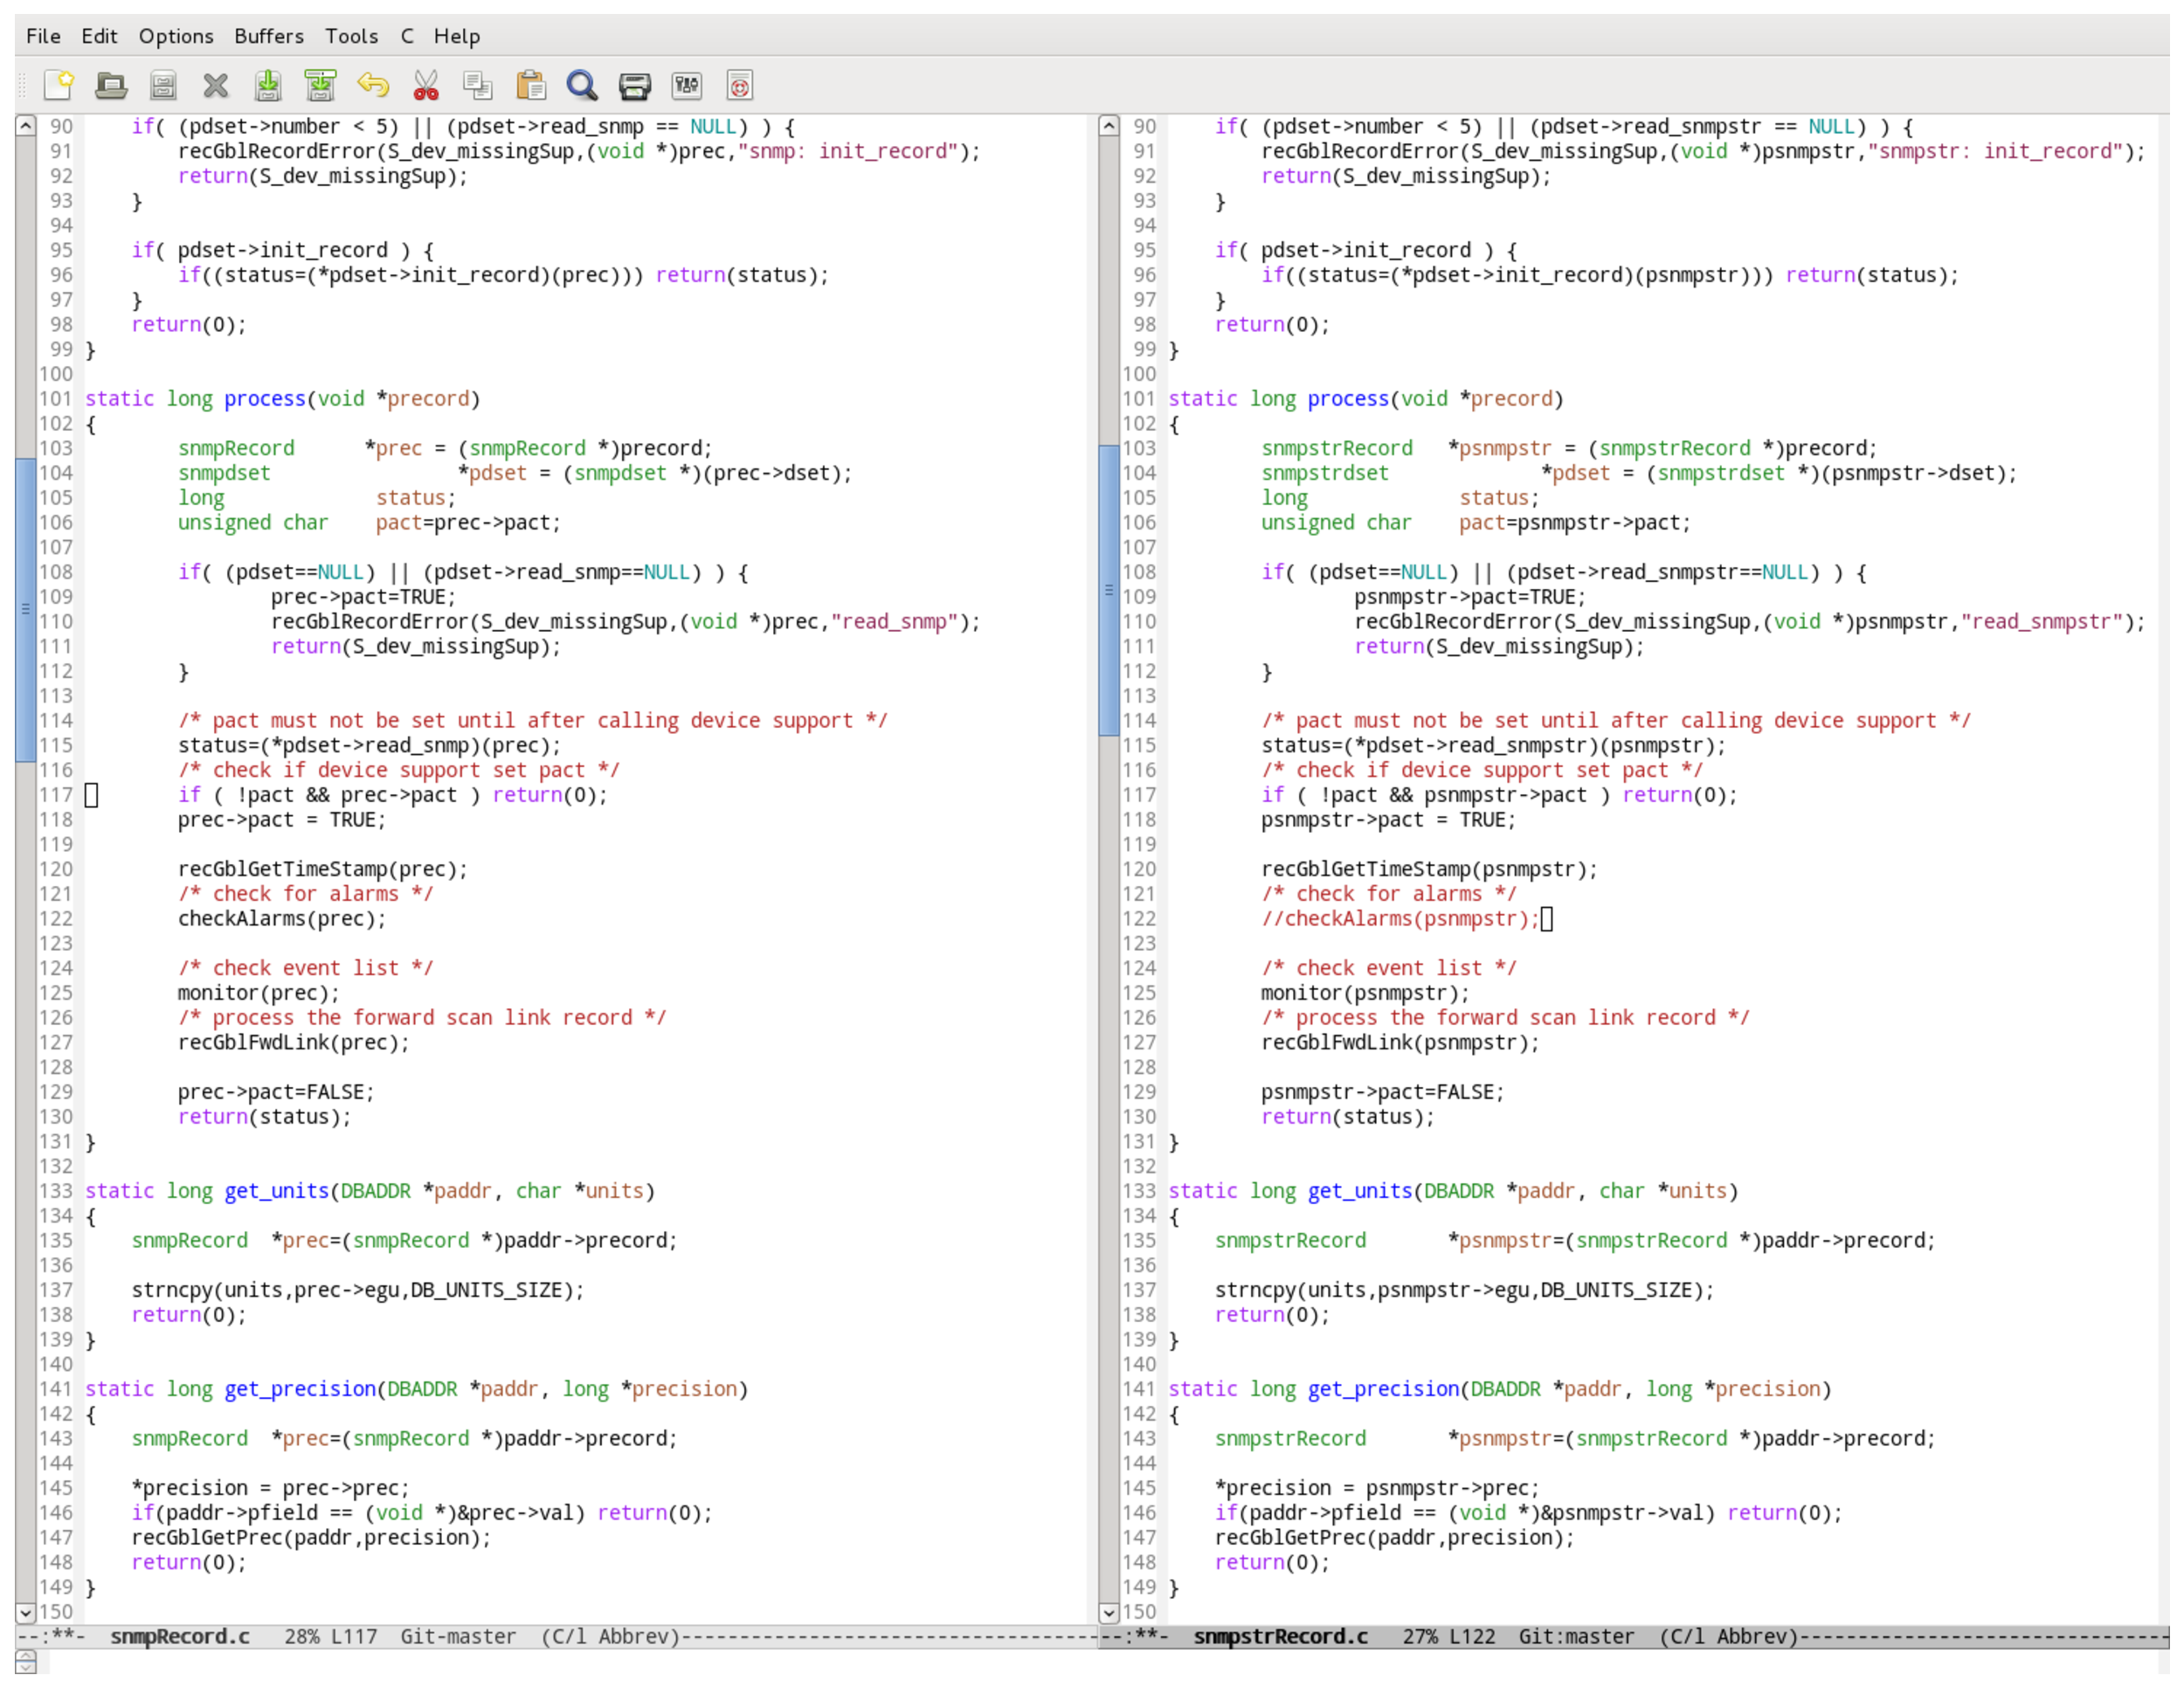
\includegraphics[width=0.89\textwidth]{./images/recordc.eps}
  \caption{record.c 파일 (left: snmpReocrd.c right: snmpstrRecord.c)}
  \label{fig:recordc}   
\end{figure}

\subsection{소스파일}
AsyncApp의 소스코드는 EPICS 환경에 맞춰 수정이 필요하다. 몇 가지 주요 수정 사항은 아래와 같고, 나머지 코드는 APPENDIX를 참조 바란다.
\begin{enumerate}
\item AsyncApp의 코드와 달리 host, community, oids는 필드로 사용되므로 OID정보와 snmp session, pdu, record 등에 대한 값은 snmp\_info의 구조로 정의한다.

\begin{lstlisting}[style=termstyle]
/*
 * a list of variables to query for
 */
struct oid_info {
  char Name[81];
  oid Oid[MAX_OID_LEN];
  unsigned int OidLen;
};

typedef struct oid_info OID;
typedef struct snmp_info
{
  OID  oid_info;
  struct snmp_session *sess;
  struct snmp_session ss;
  struct snmp_pdu *getreq;                           /* startup all hosts */
  struct snmp_pdu *setreq;                           /* startup all hosts */
  char sval[12];
  char type;
  epicsMutexId mutexId;
  void *psnmpRecord;
  void *psnmpstrRecord;
} SNMP_INFO;
\end{lstlisting}

\item devSNMPSoft, devSNMPSoftstr을 위한 dset(Address of Device Support Entry Table)을 생성한다.

\begin{lstlisting}[style=termstyle]
typedef struct devSNMPSoft{
  long number;
  DEVSUPFUN report;
  DEVSUPFUN init;
  DEVSUPFUN init_record;
  DEVSUPFUN get_ioint_info;
  DEVSUPFUN read_write_record;
  DEVSUPFUN special_linconv;
}devSNMPSoft;

typedef struct devSNMPSoftstr{
  long number;
  DEVSUPFUN report;
  DEVSUPFUN init;
  DEVSUPFUN init_record;
  DEVSUPFUN get_ioint_info;
  DEVSUPFUN read_write_record;
  DEVSUPFUN special_linconv;
}devSNMPSoftstr;

devSNMPSoft devSNMPRead = {6, NULL, NULL, snmp_RInit, NULL, snmp_Read, NULL};
devSNMPSoft devSNMPWrite = {6, NULL, NULL, snmp_WInit, NULL, snmp_Write, NULL};
epicsExportAddress(dset, devSNMPRead);
epicsExportAddress(dset, devSNMPWrite);
devSNMPSoftstr devSNMPRead_str = {6, NULL, NULL, snmp_strInit, NULL, snmp_strRead, NULL};
epicsExportAddress(dset, devSNMPRead_str);
\end{lstlisting}

\item initialize에 SNMP의 기본 정보와 SNMPv3의 인증과 암호화 부분을 추가한다. 

\begin{lstlisting}[style=termstyle]
void initializeR(void *precord)
{
  snmpRecord *psnmp = (snmpRecord *)precord;
  SNMP_INFO *snmpinfo = (SNMP_INFO*)psnmp->dpvt;

  static int snmpInited = FALSE;
  snmpinfo->oid_info.OidLen = MAX_OID_LEN;
  if (!snmpInited)
    {
      init_snmp("snmpDevAsync.c");                    /* initialize library */
      snmpInited = TRUE;
    };

  if (strlen(psnmp->vers) == 14) {                    /* VERSION 3 */
    snmp_sess_init(&(snmpinfo->ss));                  /* initialize session */    
    snmpinfo->ss.version = SNMP_VERSION_3;
    snmpinfo->ss.peername = strdup(psnmp->host);
    snmpinfo->ss.securityName =  strdup(psnmp->comm);
    snmpinfo->ss.securityNameLen = strlen((char*)snmpinfo->ss.securityName);
    snmpinfo->ss.securityLevel = SNMP_SEC_LEVEL_AUTHPRIV;

    /* Authentication Protocol */
    /* MD5 */
    snmpinfo->ss.securityAuthProto = usmHMACMD5AuthProtocol;
    snmpinfo->ss.securityAuthProtoLen = sizeof(usmHMACMD5AuthProtocol)/sizeof(oid);
    snmpinfo->ss.securityAuthKeyLen = USM_AUTH_KU_LEN;

    /* Authentication keys generation */
    if (generate_Ku(snmpinfo->ss.securityAuthProto,
		    snmpinfo->ss.securityAuthProtoLen,
		    (u_char *) strdup(psnmp->auth), strlen(psnmp->auth),
		    snmpinfo->ss.securityAuthKey,
		    &snmpinfo->ss.securityAuthKeyLen) != SNMPERR_SUCCESS) {
      snmp_perror("Error!!!!!!!!!!!!");
      snmp_log(LOG_ERR,
	       "Error generating Ku from authentication pass phrase. \n");
      exit(1);
    }

    /* Privacy protocol */
    /* DES */
    snmpinfo->ss.securityPrivProto = usmDESPrivProtocol;
    snmpinfo->ss.securityPrivProtoLen = USM_PRIV_PROTO_DES_LEN;
    snmpinfo->ss.securityPrivKeyLen = USM_PRIV_KU_LEN;

    /* Privacy keys generation */
    if (generate_Ku(snmpinfo->ss.securityAuthProto,
		    snmpinfo->ss.securityAuthProtoLen,
		    (u_char *) strdup(psnmp->priv), strlen(psnmp->priv),
		    snmpinfo->ss.securityPrivKey,
		    &snmpinfo->ss.securityPrivKeyLen) != SNMPERR_SUCCESS) {
      printf ("Error generating Ku from privacity pass phrase. \n");
      exit(1);
    }

    snmpinfo->ss.callback = asynch_response;        /* default callback */
    snmpinfo->ss.callback_magic = snmpinfo;
  } else {                                          /* VERSION 2c */
    snmp_sess_init(&(snmpinfo->ss));                /* initialize session */
    snmpinfo->ss.version = SNMP_VERSION_2c;
    snmpinfo->ss.peername = strdup(psnmp->host);
    snmpinfo->ss.community = (unsigned char*)strdup(psnmp->comm);
    snmpinfo->ss.community_len = strlen((char*)snmpinfo->ss.community);
    snmpinfo->ss.callback = asynch_response;        /* default callback */
    snmpinfo->ss.callback_magic = snmpinfo;
  }
  
                                                    /* parse the oids */
  if (!read_objid(psnmp->oids, snmpinfo->oid_info.Oid, &snmpinfo->oid_info.OidLen))      
    {
      printf("parse the oids %s\n",psnmp->oids);
      snmp_perror("read_objid");
      exit(1);
    }
}
\end{lstlisting}

\item Switch문을 사용하여 SNMP 데이터 타입에 따라 callback 되는 데이터값을 처리한다.

\begin{lstlisting}[style=termstyle]
int return_data(int status, struct snmp_info *sinfo, struct snmp_pdu *pdu)               
{
  char buf[1024];
  struct variable_list *vp;
  int ix;
  char *getdata = NULL;
  int nVal;
  char tVal[40];
  char *sVal;
  char *pValStr;
  struct snmp_session *sp = sinfo->sess;
  snmpRecord *psnmp = (snmpRecord *)sinfo->psnmpRecord;
  snmpstrRecord *psnmpstr = (snmpstrRecord *)sinfo->psnmpstrRecord;

  switch (status) {
  case STAT_SUCCESS:
    vp = pdu->variables;
    if (pdu->errstat == SNMP_ERR_NOERROR) {
      while (vp) {
	snprint_variable(buf, sizeof(buf), vp->name, vp->name_length, vp);
	/*mjpark------------------------------------------*/
	pValStr = strrchr(buf, ':');
	sprintf(tVal, "%s", pValStr+2);
	getdata = (char *)malloc(1 + vp->val_len);
	memcpy(getdata, vp->val.string, vp->val_len);
	getdata[vp->val_len] = '\0';
	sVal = trimwhitespace(replace_str2(tVal,"\"","")); 

	switch(vp->type)
	  {
	  case ASN_INTEGER:
	    {
	      memcpy((void *)&nVal, getdata, sizeof(int));
	      psnmp->val = nVal;
	      break;
	    }
	  case ASN_OCTET_STR:
	  case ASN_BIT_STR:
	    {
	      sprintf(psnmpstr->val, "%s", sVal);
	      break;
	    }
	  case ASN_GAUGE:
	  case ASN_OPAQUE:
	  case ASN_COUNTER:
	  case ASN_TIMETICKS:
	  case ASN_IPADDRESS:
	  default :
	    sscanf(tVal,"%lg",&psnmp->val);
	  }
	/*------------------------------------------------*/
	vp = vp->next_variable;
      }
      free(getdata);
    }
    else {
      for (ix = 1; vp && ix != pdu->errindex; vp = vp->next_variable, ix++);
      if (vp)
	snprint_objid(buf, sizeof(buf), vp->name, vp->name_length);
      else
	strcpy(buf, "(none)");
      fprintf(stdout, "%s: %s: %s\n", sp->peername, buf, snmp_errstring(pdu->errstat));
    }
    return 1;
    
  case STAT_TIMEOUT:
    fprintf(stdout, "%s: Timeout\n", sp->peername);
    return 0;
  
  case STAT_ERROR:
    snmp_perror(sp->peername);
    return 0;
  }
  return 0;
}
\end{lstlisting}

\item 제어를 위해 AsyncApp에 없는 snmpset을 추가한다.

\begin{lstlisting}[style=termstyle]
int set_snmp(void *precord, const char *sval)
{
  snmpRecord *psnmp = (snmpRecord *)precord;
  SNMP_INFO *snmpinfo = (SNMP_INFO*)psnmp->dpvt;
  char type = 'i';

  if (!(snmpinfo->sess = snmp_open(&snmpinfo->ss))) {
    snmp_perror("snmp_open");
    return -1;
  };
  
  static int count = 0;
  printf("SValue[%d]: %s\n", count++, sval);

  snmpinfo->setreq = snmp_pdu_create(SNMP_MSG_SET);   /* send the first GET */
  if (! snmpinfo->setreq) {
    snmp_free_pdu(snmpinfo->setreq);
    snmp_close(snmpinfo->sess);                       /* cleanup */
    return -1;
  }
  
/* snmp_add_var(netsnmp_pdu *, const oid *, size_t, char, const char *) */
  snmp_add_var(snmpinfo->setreq, snmpinfo->oid_info.Oid, snmpinfo->oid_info.OidLen, type, sval);       

  if (snmp_send(snmpinfo->sess, snmpinfo->setreq))
    hosts++;
  else {
    snmp_perror("snmp_setsend");
    snmp_free_pdu(snmpinfo->setreq);
    snmp_close(snmpinfo->sess);                      /* cleanup */
    return -1;
  }

  active_hosts();
  snmp_close(snmpinfo->sess);                        /* cleanup */
  return 0;
}
\end{lstlisting}
\end{enumerate}

\subsection{dbd}
코드가 작성되면 dset에 맞춰 dbd파일을 작성한다.


\begin{lstlisting}[style=termstyle]
include "snmpRecord.dbd"
include "snmpstrRecord.dbd"

device(snmp,INST_IO,devSNMPRead,"SNMP Read")
device(snmp,INST_IO,devSNMPWrite,"SNMP Write")
device(snmpstr,INST_IO,devSNMPRead_str,"SNMP Read")
\end{lstlisting}

\subsection{Makefile}
위의 과정을 거쳐 수정 및 생성한 파일들을 라이브러리로 만들어 EPICS IOC에서 실행하기 위해 Makefile을 수정한다. 라이브러리로 사용할 이름을 설정하고, 빌드할 파일들을 설정한다.

\begin{lstlisting}[style=termstylenumber]
TOP = ../..
include $(TOP)/configure/CONFIG

LIBRARY += snmpMon
DBDINC       += snmpRecord snmpstrRecord
DBD          += snmpRecord.dbd snmpstrRecord.dbd
DBD          += snmpDevSoft.dbd
snmpMon_SRCS += snmpDevAsync.c snmpRecord.c snmpstrRecord.c

netsnmp_DIR = /usr/lib
# for jessie, need to check for Wheezy
# jhlee
netsnmp_DIR += /usr/lib/x86_64-linux-gnu
snmpMon_LIBS +=netsnmp

# need to check where it is in Wheezy

USR_CFLAGS  += `net-snmp-config --cflags`
USR_LDFLAGS += `net-snmp-config --libs`
PROD_LDLIBS += `net-snmp-config --libs`

include $(TOP)/configure/RULES      
\end{lstlisting}

Makefile 수정 후 make를 실행하면 아래와 같이 lib, include, dbd폴더와 파일들이 생성된다.

    {\scriptsize
         \begin{verbatim}
    
mijoy0909@mjpark:~/epics/R3.14.12.4/siteLibs$ tree -L 3

├── [       4096]  dbd
│   ├── [        445]  snmpDevSoft.dbd
│   ├── [       5926]  snmpRecord.dbd
│   └── [       3024]  snmpstrRecord.dbd
├── [       4096]  include
│   ├── [      19578]  snmpRecord.h
│   └── [      14389]  snmpstrRecord.h
├── [       4096]  lib
│   └── [       4096]  linux-x86_64
│       ├── [     165542]  libsnmpMon.a
│       └── [     103574]  libsnmpMon.so
├── [        186]  Makefile
├── [        345]  Makefile.template
├── [       4096]  README
├── [       4096]  snmpLib
│   ├── [        305]  Makefile
│   ├── [       4096]  mibs
│   ├── [       4096]  rawcode
│   └── [       4096]  src
│       ├── [        628]  Makefile
│       ├── [       4096]  O.Common
│       ├── [       4096]  O.linux-x86_64
│       ├── [      27789]  snmpDevAsync.c
│       ├── [        445]  snmpDevSoft.dbd
│       ├── [       7086]  snmpRecord.c
│       ├── [       5926]  snmpRecord.dbd
│       ├── [       7803]  snmpstrRecord.c
│       ├── [       3024]  snmpstrRecord.dbd
└──     └── [       4096]  test
     \end{verbatim}
     }

\section{Application 구성}
만들어진 Library를 사용하여 EPICS IOC를 실행하기 위한 Application을 구성한다.

\subsection{Application 환경 폴더생성}
Application 구성을 위해 EPICS에서 제공되는 makeBaseApp.pl을 사용하여 Application 환경폴더를 생성한다.

\begin{lstlisting}[style=termstyle]
mijoy0909@mjpark:~/epics/R3.14.12.4/siteApps/snmp2$ makeBaseApp.pl -t ioc snmp2
mijoy0909@mjpark:~/epics/R3.14.12.4/siteApps/snmp2$ makeBaseApp.pl -i -t ioc snmp2
Using target architecture linux-x86_64 (only one available)
The following applications are available: snmp2
What application should the IOC(s) boot?
The default uses the IOC's name, even if not listed above.
Application name? snmp2
mijoy0909@mjpark:~/epics/R3.14.12.4/siteApps/snmp2$ ls
configure/  iocBoot/  Makefile  snmp2App/
\end{lstlisting}

Application 환경을 만든 후 make를 하면 아래와 같이 bin, dbd 폴더가 생성된다.
\begin{lstlisting}[style=termstyle]
mijoy0909@mjpark:~/epics/R3.14.12.4/siteApps/snmp2$ make
mijoy0909@mjpark:~/epics/R3.14.12.4/siteApps/snmp2$ ls
bin/  configure/  dbd/  iocBoot/  Makefile  snmp2App/
\end{lstlisting}

\subsection{src/Makefile 수정}
환경을 구성한 후 앞서 만든 library를 사용하기 위해 siteApps/snmp2/snmp2App/src/Makefile을 수정한다.

\begin{lstlisting}[style=termstylenumber]
TOP=../..

include $(TOP)/configure/CONFIG


USR_INCLUDES += -I${RAON_SITELIBS}/include/
USR_DBDFLAGS += -I${RAON_SITELIBS}/dbd/
USR_INCLUDES  += -I$(EPICS_EXTENSIONS)/include

snmpMon_DIR += ${RAON_SITELIBS}/lib/$(T_A)

#----------------------------------------
#  ADD MACRO DEFINITIONS AFTER THIS LINE
#=============================

#=============================
# Build the IOC application

PROD_IOC = snmp2
# snmp2.dbd will be created and installed
DBD += snmp2.dbd

# snmp2.dbd will be made up from these files:
snmp2_DBD += base.dbd
snmp2_DBD += snmpRecord.dbd

# Include dbd files from all support applications:
#snmp2_DBD += xxx.dbd
snmp2_DBD += snmpDevSoft.dbd

# Add all the support libraries needed by this IOC
#snmp2_LIBS += xxx
snmp2_LIBS += snmpMon 


# snmp2_registerRecordDeviceDriver.cpp derives from snmp2.dbd
snmp2_SRCS += snmp2_registerRecordDeviceDriver.cpp

# Build the main IOC entry point on workstation OSs.
snmp2_SRCS_DEFAULT += snmp2Main.cpp
snmp2_SRCS_vxWorks += -nil-

# Add support from base/src/vxWorks if needed
#snmp2_OBJS_vxWorks += $(EPICS_BASE_BIN)/vxComLibrary

# Finally link to the EPICS Base libraries
snmp2_LIBS += $(EPICS_BASE_IOC_LIBS)

#===========================

include $(TOP)/configure/RULES
#----------------------------------------
#  ADD RULES AFTER THIS LINE
\end{lstlisting}

\subsection{db파일 생성}
EPIC IOC를 통해 모니터링 및 제어를 원하는 장비의 MIB정보를 record로 만들어 db파일을 생성한다. 아래는 WIENER Crate db파일의 예이다. 레코드의 Read/Write여부를 결정하고, 그에 맞춰 버전과 인증비밀번호, Host, Communiy, OID의 정보를 필드로 추가한다.

\begin{lstlisting}[style=termstyle]
record(snmp, "${W}:${C}_MainPower_W") {
  field(DESC, "WIENER Main Power Switch") 
  field(DTYP, "SNMP Write")
  field(SCAN, "5 second")
  field(VERS, "${V3}")
  field(AUTH, "${AUTH_P}")
  field(PRIV, "${PRIV_P}")
  field(HOST, "${HOST}")
  field(COMM, "${USER}")
  field(OIDS, "${WI}sysMainSwitch.0")
  field(MDEL, "-1")
  field(RVAL, "1")
}

record(snmp, "${W}:${C}_MainPower_R") {
  field(DESC, "WIENER Main Power Switch") 
  field(DTYP, "SNMP Read")
  field(SCAN, "5 second")
  field(VERS, "${V2C}")
  field(HOST, "${HOST}")
  field(COMM, "${COM}")
  field(OIDS, "${WI}sysMainSwitch.0")
  field(MDEL, "-1")
}
\end{lstlisting}

\subsection{Db/Makefile 수정}
생성된 db파일을 사용하기 위해 siteApps/snmp2/snmp2App/Db의 Makefile을 수정한다.

\begin{lstlisting}[style=termstylenumber]
TOP=../..
include $(TOP)/configure/CONFIG
#----------------------------------------
#  ADD MACRO DEFINITIONS AFTER THIS LINE

#----------------------------------------------------
#  Optimization of db files using dbst (DEFAULT: NO)
#DB_OPT = YES

#----------------------------------------------------
# Create and install (or just install) into <top>/db
# databases, templates, substitutions like this
#DB += xxx.db
DB += wiener.vdb

#----------------------------------------------------
# If <anyname>.db template is not named <anyname>*.template add
# <anyname>_template = <templatename>

include $(TOP)/configure/RULES
#----------------------------------------
#  ADD RULES AFTER THIS LINE
\end{lstlisting}

\subsection{IOC 실행}
EPICS IOC 실행에 앞서 siteApps/snmp2에서 make를 실행한다. 실행 후 문제가 없다면 iocBoot/iocsnmp2로 이동하여 st.cmd에 db파일을 추가한다.

\begin{lstlisting}[style=termstylenumber]
#!../../bin/linux-x86_64/snmp2

## You may have to change snmp2 to something else
## everywhere it appears in this file

< envPaths

cd ${TOP}

epicsEnvSet("MIBDIRS", "${EPICS_PATH}/siteLibs/snmpLib/mibs")

## Register all support components
dbLoadDatabase "dbd/snmp2.dbd"
snmp2_registerRecordDeviceDriver pdbbase

## Load record instances
#dbLoadRecords("db/xxx.db","user=mijoy0909Host")
dbLoadRecords("db/wiener.vdb", "W=WIENER, C=CRATE3, HOST=10.1.5.123, COM=public, USER=admin, V2C=SNMP_VERSION_2c, V3=SNMP_VERSION_3, WI=WIENER-CRATE-MIB::, AUTH_P=MySecret, PRIV_P=MySecret")

cd ${TOP}/iocBoot/${IOC}
iocInit

## Start any sequence programs
#seq sncxxx,"user=mijoy0909Host"
\end{lstlisting}

위의 과정이 모두 완료되면 st.cmd에 실행권한을 부여하고 실행시킨다.

\begin{lstlisting}[style=termstyle]
mijoy0909@mjpark:~/epics/R3.14.12.4/siteApps/snmp2/iocBoot/iocsnmp2$ chmod 755 st.cmd
\end{lstlisting}

EPICS IOC 실행 결과는 다음과 같다.

\begin{lstlisting}[style=termstyle]
mijoy0909@mjpark:~/epics/R3.14.12.4/siteApps/snmp2/iocBoot/iocsnmp2$ ./st.cmd 
#!../../bin/linux-x86_64/snmp2
## You may have to change snmp2 to something else
## everywhere it appears in this file
< envPaths
epicsEnvSet("ARCH","linux-x86_64")
epicsEnvSet("IOC","iocsnmp2")
epicsEnvSet("TOP","/home/mijoy0909/epics/R3.14.12.4/siteApps/snmp2")
cd /home/mijoy0909/epics/R3.14.12.4/siteApps/snmp2
#epicsEnvSet("MIBDIRS", "${EPICS_PATH}/siteLibs/snmpLib/mibs")
## Register all support components
dbLoadDatabase "dbd/snmp2.dbd"
snmp2_registerRecordDeviceDriver pdbbase
#drvSNMPConnInit("10.1.5.142", "qwertyuiop12345", "qwertyuiop12345");
#drvSNMPConnInit("SNMP_VERSION_2c", "10.1.5.142", "public", NULL, NULL);
## Load record instances
#dbLoadRecords("db/xxx.db","user=mijoy0909Host")
dbLoadRecords("db/pdu.vdb", "A=APC, P=PDU2, HOST=10.1.5.142, COM=public, USER=mijoy, V2C=SNMP_VERSION_2c, V3=SNMP_VERSION_3, PO=PowerNet-MIB::, AUTH_P=qwertyuiop12345, PRIV_P=qwertyuiop12345")
dbLoadRecords("db/wiener.vdb", "W=WIENER, C=CRATE3, HOST=10.1.5.123, COM=public, USER=admin, V2C=SNMP_VERSION_2c, V3=SNMP_VERSION_3, WI=WIENER-CRATE-MIB::, AUTH_P=MySecret, PRIV_P=MySecret")
dbLoadRecords("db/timestamp.vdb", "S=SNMPIOC")
cd /home/mijoy0909/epics/R3.14.12.4/siteApps/snmp2/iocBoot/iocsnmp2
iocInit
Starting iocInit
############################################################################
## EPICS R3.14.12.4 $Date: Mon 2013-12-16 15:51:45 -0600$
## EPICS Base built Aug 29 2014
############################################################################
iocRun: All initialization complete
## Start any sequence programs
#seq sncxxx,"user=mijoy0909Host"
epics> 
epics> dbl
WIENER:CRATE3_MainPower_R
WIENER:CRATE3_MainPower_W
\end{lstlisting}


\clearpage
\bibliographystyle{unsrtnat}
\bibliography{./refs}




\end{document}
